% ******************************************************** %
%              TEMPLATE DE INFORME ORGA2 v0.1              %
% ******************************************************** %
% ******************************************************** %
%                                                          %
% ALGUNOS PAQUETES REQUERIDOS (EN UBUNTU):                 %
% ========================================
%                                                          %
% texlive-latex-base                                       %
% texlive-latex-recommended                                %
% texlive-fonts-recommended                                %
% texlive-latex-extra?                                     %
% texlive-lang-spanish (en ubuntu 13.10)                   %
% ******************************************************** %


\documentclass[a4paper]{article}
\usepackage[spanish]{babel}
\usepackage[utf8]{inputenc}
\usepackage{charter}   % tipografia
\usepackage{graphicx}
%\usepackage{makeidx}
\usepackage{paralist} %itemize inline
\usepackage{subcaption}


%\usepackage{float}
%\usepackage{amsmath, amsthm, amssymb}
%\usepackage{amsfonts}
%\usepackage{sectsty}
%\usepackage{charter}
%\usepackage{wrapfig}
%\usepackage{listings}
%\lstset{language=C}

% \setcounter{secnumdepth}{2}
\usepackage{underscore}
\usepackage{caratula}
\usepackage{url}
\usepackage{ragged2e}
\usepackage{hyperref}
\usepackage{pdfpages}


% ********************************************************* %
% ~~~~~~~~              Code snippets             ~~~~~~~~~ %
% ********************************************************* %

\usepackage{color} % para snipets de codigo coloreados
\usepackage{fancybox}  % para el sbox de los snipets de codigo

\definecolor{litegrey}{gray}{0.94}

\newenvironment{codesnippet}{%
	\begin{Sbox}\begin{minipage}{\textwidth}\sffamily\small}%
	{\end{minipage}\end{Sbox}%
		\begin{center}%
		\vspace{-0.4cm}\colorbox{litegrey}{\TheSbox}\end{center}\vspace{0.3cm}}



% ********************************************************* %
% ~~~~~~~~         Formato de las páginas         ~~~~~~~~~ %
% ********************************************************* %

\usepackage{fancyhdr}
\pagestyle{fancy}

%\renewcommand{\chaptermark}[1]{\markboth{#1}{}}
\renewcommand{\sectionmark}[1]{\markright{\thesection\ - #1}}

\fancyhf{}

\fancyhead[LO]{Sección \rightmark} % \thesection\ 
\fancyfoot[LO]{\small{Ivo Pajor, Laureano Muñiz, Luciana Gorosito}}
\fancyfoot[RO]{\thepage}
\renewcommand{\headrulewidth}{0.5pt}
\renewcommand{\footrulewidth}{0.5pt}
\setlength{\hoffset}{-0.8in}
\setlength{\textwidth}{16cm}
%\setlength{\hoffset}{-1.1cm}
%\setlength{\textwidth}{16cm}
\setlength{\headsep}{0.5cm}
\setlength{\textheight}{25cm}
\setlength{\voffset}{-0.7in}
\setlength{\headwidth}{\textwidth}
\setlength{\headheight}{13.1pt}

\renewcommand{\baselinestretch}{1.1}  % line spacing

% ******************************************************** %


\begin{document}


\thispagestyle{empty}
\materia{Organización del Computador II}
\submateria{Segundo Cuatrimestre de 2020}
\titulo{Trabajo Práctico II}
\subtitulo{Procesamiento de imágenes (SIMD)}
\integrante{Ivo Pajor}{460/19}{ivo_pajor@hotmail.com}
\integrante{Laureano Muñiz}{498/19}{lau2000m@hotmail.com}
\integrante{Luciana Gorosito}{577/18}{lugorosito0@gmail.com}

\maketitle
\newpage

\thispagestyle{empty}
\vfill


\thispagestyle{empty}
\vspace{3cm}
\tableofcontents
\newpage


%\normalsize
\newpage

\section{Introducción}

\justify
El objetivo de este Trabajo Práctico es analizar y comprender el modelo de procesamiento SIMD \textit{(Single Instruction, Multiple Data)} y su relación con la microarquitectura del procesador, mediante la implementación en lenguaje ensamblador de tres filtros gráficos: <<\textit{Imagen Fantasma}>>, <<\textit{Color Bordes}>> y <<\textit{Reforzar Brillo}>>. 
\justify
Más detalladamente, el filtro <<\textit{Imagen Fantasma}>> combina una imagen original con su versión en escala de grises y del doble de tamaño, generando así un  efecto de imagen fantasma sobre la imagen destino. El filtro <<\textit{Color Bordes}>> detecta los bordes de una  imagen y el filtro <<\textit{Reforzar Brillo}>> modifica el brillo de una imagen, aumentándolo en el caso de que  supere al valor del parámetro \textit{umbralSup} y disminuyéndolo en el caso de que esté por debajo del valor  del parámetro \textit{umbralInf}.
\justify
\indent Las implementaciones de estos filtros se realizaron utilizando el set de instrucciones \textbf{SSE} y técnicas de programación vectorial, que permitieron procesar en paralelo de 2 a 4 píxeles, dependiendo del filtro. Posterior a la implementación se realizó un análisis de rendimiento en comparación a las implementaciones en lenguaje C, provistas por la cátedra. Además, se diseñaron dos experimentos motivados en entender las posibles causas de la variación del rendimiento y la limitación de la performance de los algoritmos en el procesamiento de imágenes, que serán detallados en las secciones siguientes.  


\section{Desarrrollo}

\subsection{Implementaciones en ASM}
\justify
En esta sección se incluyen las descripciones de las funciones implementadas en lenguaje ensamblador.

\subsubsection{Imagen Fantasma}
\justify
En primer lugar, se definieron en la sección \textit{section .data} los offset necesarios para obtener los parámetros que fueron pasados por la pila (offset_x y offset_y) y las máscaras a utilizar en la operatoria con los píxeles, estas son:
\begin{itemize}
	\item \textit{transparencia}: máscara utilizada para borrar la componente de transparencia del píxel, la misma fue luego restaurada al terminar el ciclo usando la máscara \textit{sumar}.
	\item \textit{green}: máscara utilizada para extraer la componente G del píxel, ya que es la única componente que duplica su valor al calcularse el brillo.
	\item \textit{multiplicar}: máscara utilizada para multiplicar por $29$, ya que $\frac{29}{32} \cong $ 0.9, en la conversión a escala de grises.
	\item \textit{sumar}: máscara utilizada para arreglar las transparencias de los píxeles al finalizar los cálculos.
	
 Previo al inicio del ciclo, se calculó el offset en bytes correspondiente al píxel de la posición (jj,ii) de la imagen Fuente, del cual se obtiene el brillo. La idea principal de este algoritmo es recorrer a la imagen en submatrices de 2x2, levantando de memoria en los registros \textit{xmm1 y xmm2}  los píxeles que les corresponde el mismo valor de brillo, para así poder procesarlos en paralelo.
 \begin{figure}[h]
 	\centering
 	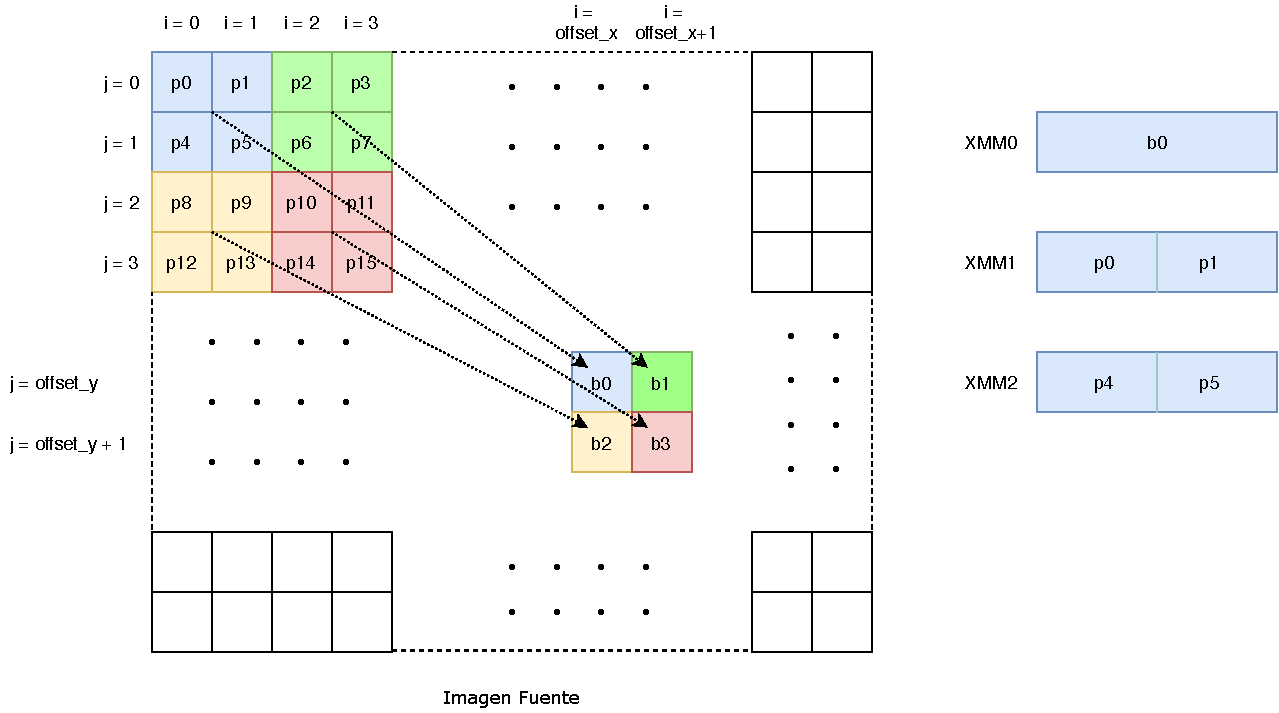
\includegraphics[scale = 0.6]{img/ImagenFantasma1.pdf}
 	\caption{Levantamiento de memoria Imagen Fantasma}
 \end{figure}
 
 Más específicamente, en cada iteración del ciclo se realizaron los siguientes pasos:
 
 \begin{enumerate}
 	\item \textbf{Cálculo de brillo}\\
 	Se levanta el píxel src[jj][ii] en el registro \textit{xmm0}, extendiendo con ceros cada componente a dword, para poder realizar cálculos sin perder precisión. Además, como el cálculo del  brillo solo necesita de las componentes RGB del píxel, antes de proceder se setea en cero a la componente A, aplicando la máscara \textit{transparencia} antes mencionada. Seguido a esto, se extrae en el registro \textit{xmm13} la componente G del píxel, aplicando la máscara \textit{green}. Se sumaron los registros \textit{xmm0} y \textit{xmm13}, y se realizaron dos sumas horizontales consecutivas del registro \textit{xmm0}, obteniéndose en las cuatro \textit{dwords} de este registro el resultado de la operación:
 	\begin{equation}
 	4B = src[jj][ii].r + 2 * src[jj][ii].g + src[jj][ii].b 
 	\end{equation}
 	Para finalizar el cálculo de brillo se transforman las \textit{dwords} a \textit{words} saturando de manera \textit{unsigned}. Por último, resta dividir por $4$. Como en la conversión a escala de grises se utiliza el valor de $\frac{B}{2}$ se dividen por $8$ las \textit{words} del registro \textit{xmm0} utilizando operaciones de shifteo hacia derecha.
 	
 \begin{figure}[h]
 	\centering
 	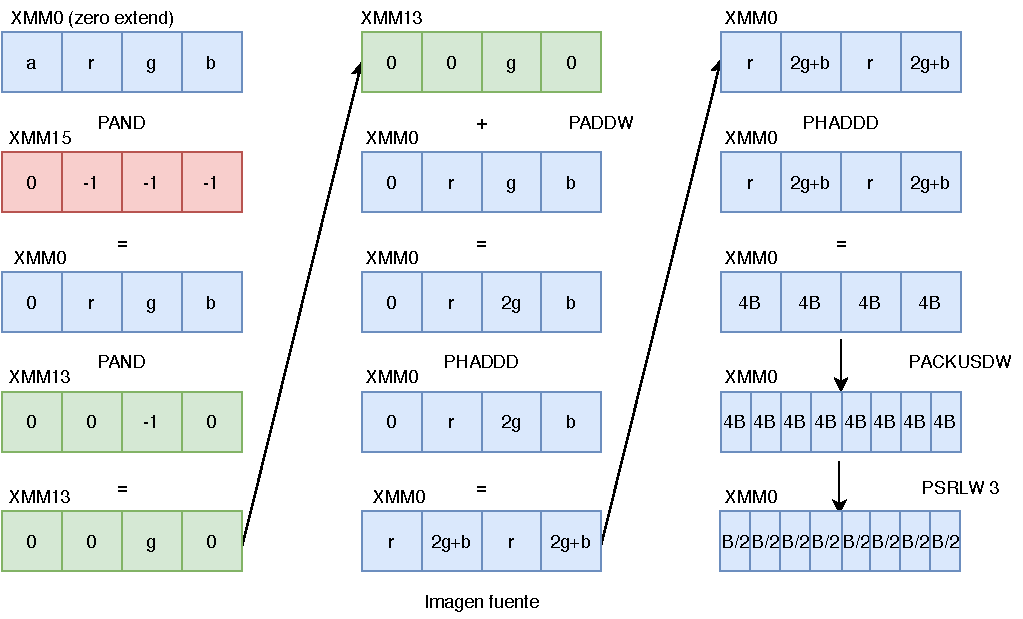
\includegraphics[scale = 0.6]{img/ImFan21.pdf}
 	\caption{Operatoria del cálculo de brillo}
 \end{figure}
 
 
 	\item \textbf{Conversión a escala de grises}\\
 	
 	Se levantan los píxeles de la submatriz de 2x2 en los registros \textit{xmm1 y xmm2}, extendiendo sin signo de \textit{byte} a \textit{word}. Se multiplican los valores de las componentes por $29$ utilizando la máscara \textit{multiplicar}. Luego, se shiftean las componentes hacia derecha $5$ bits, lo cual equivale a dividir por $32$ tomando piso. Por último, se suma \textit{xmm0} a ambos registros de forma saturada \textit{unsigned} para luego empaquetarlos de la  misma manera de \textit{words} a \textit{bytes}. 
 	
 	Antes de cargar los resultados en la imagen Destino, se arreglan las transparencias de los píxeles con la máscara \textit{sumar}. 
 	
 \begin{figure}[h]
 	\centering
 	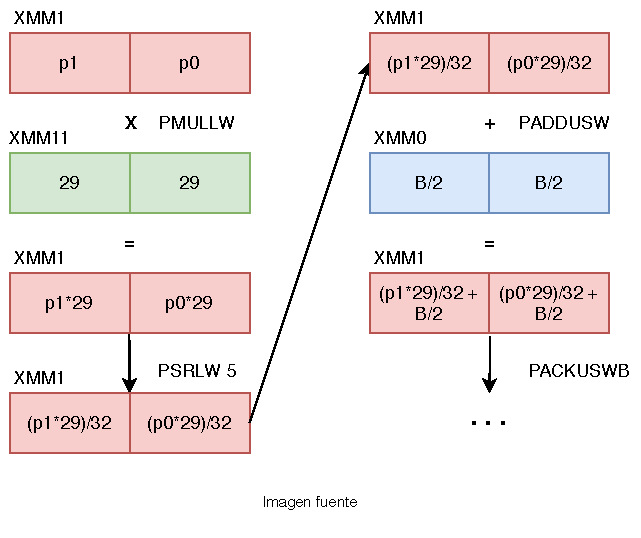
\includegraphics[scale = 0.66]{img/ImFan3.pdf}
 	\caption{Operatoria de la conversión a escala de grises}
 \end{figure}
 	
 	    
 \end{enumerate}
 
	
\end{itemize}	 

\newpage
\subsubsection{Color Bordes}
Se definieron en la sección \textit{section .data} las siguientes máscaras:

\begin{itemize}
	\item \textit{blanco}: máscara utilizada para colorear de blanco los bordes de la imagen destino.
	\item \textit{transparencias1}: máscara utilizada para restaurar la transparencia de un píxel.
	\item \textit{transparencias2}: máscara utilizada para filtrar la componente de transparencia de un píxel.	
\end{itemize}	
\justify
y, antes de comenzar el ciclo, fueron guardadas en los registros \textit{xmm15, xmm14 y xmm13}, respectivamente.


\justify
El algoritmo consta de dos ciclos cortos (\textit{".bordesPrimeraFila"} y \textit{".bordesUltimaFila"}) que arman los bordes blancos horizontales de la imagen Destino, un \textit{"preciclo"}, que actualiza las variables antes de ingresar a los otros dos ciclos (\textit{".cicloFilas"} y \textit{".cicloColumnas"}) que recorren la imagen Fuente realizando la operatoria de detección de bordes y armando los bordes verticales blancos de la imagen Destino. A continuación se detallan las operaciones que se realizan en cada parte.

\begin{itemize}
	\item \textbf{.bordesPrimeraFila}\\
	 En cada iteración del ciclo se escriben 16 bytes de la imagen Destino con el valor de 255 (correspondiente al blanco), usando la máscara previamente guardada en el registro \textit{xmm15}. Como se escriben cuatro píxeles de manera simultánea en cada iteración, el registro contador \textbf{edx} fue inicializado con el valor de $\#\frac{columnas}{4}$ y, para compensar el factor multiplicativo que le falta a la escala, el registro índice \textbf{r9d} fue incrementado en 2 unidades cada iteración.  
	
	\item \textbf{.preciclo}\\
	Se guarda en \textbf{rdi} la dirección efectiva a la posición (1,1) de la imagen Fuente y se guarda en \textbf{rsi} la dirección efectiva a la posición (1,0) de la imagen Destino. Además, se decrementa el valor del registro contador de filas \textbf{ecx}, porque la primera fila (j=0) ya fue coloreada de blanco en el primer ciclo de bordes.  
	
	\item \textbf{.cicloFila y .cicloColumnas}\\
	El ciclo externo (.cicloFilas) recorre a las imágenes Fuente y Destino por filas, empezando desde la segunda fila (j=1). La guarda del ciclo compara a \textbf{ecx} (registro contador de filas) con 1, por el margen de un píxel que debe dejarse y que es coloreado de blanco en la imagen Destino durante el último ciclo de bordes. Cada vez que se ingresa al ciclo de las filas, se pinta de blanco el primer píxel de la imagen Destino y se avanza un píxel en la misma. De esta manera se va generando el margen vertical izquierdo de esa imagen. Además, antes de ingresar al ciclo interno, se resetea el contador de columnas \textbf{eax}. El valor del contador es $\#\frac{columnas-2}{2}$, ya que los píxeles de la primera y última columna de la imagen Fuente no se procesan y 
	el resto de la operatoria se hace procesando de a 2 píxeles.\\
	En cada iteración del ciclo interno (.cicloColumnas) se levantan de memoria los doce píxeles necesarios para procesar los píxeles de la posición [rdi] y [rdi + 4]. Se levantan dos píxeles por registro, extendiendo con ceros las componentes de cada píxel de byte a word, quedando así 2 píxeles por registro \textit{xmm}. Se limpia el registro \textit{xmm6}, que es usado como registro acumulador y se reservan en otros registros los píxeles necesarios para calcular las diferencias verticales.
	\begin{figure}[h]
		\centering
		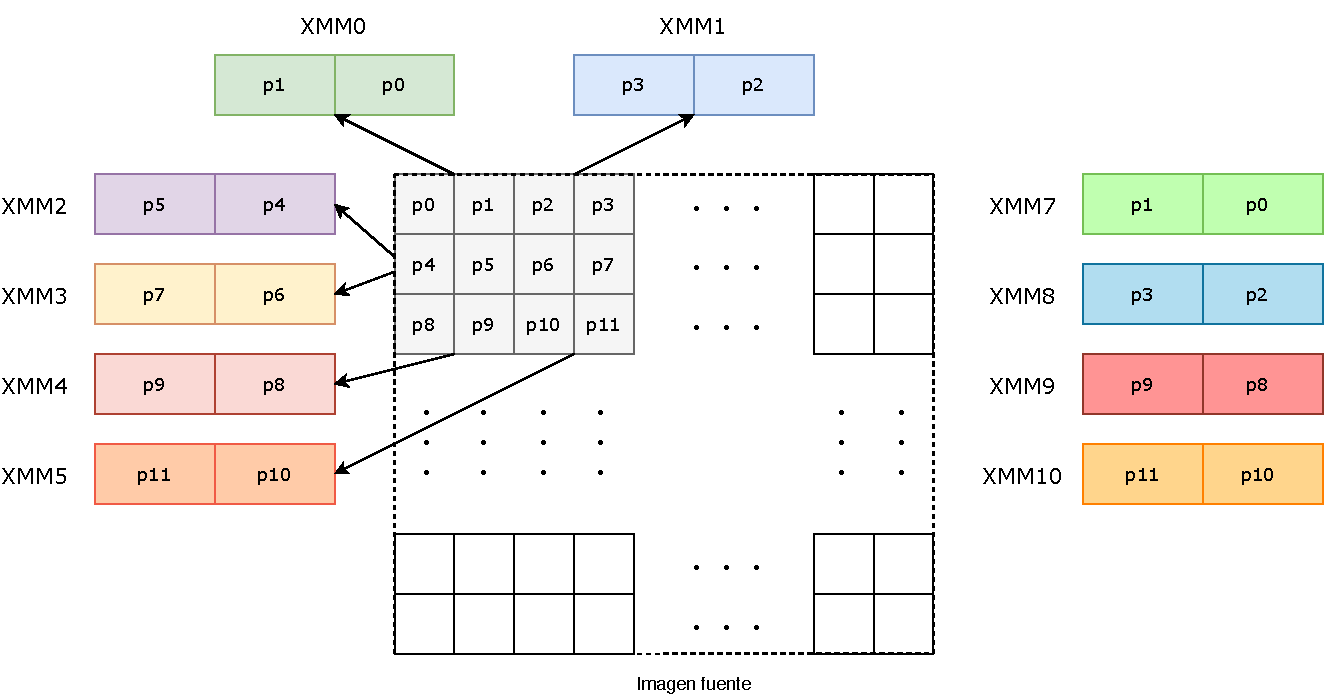
\includegraphics[scale=0.6]{img/LevColorBordes.pdf}
		\caption{Levantamiento de memoria Color Bordes}
	\end{figure}
	
	Para calcular las diferencias horizontales, se restan los registros correspondientes a una misma fila y luego se toma valor absoluto. El resultado de cada diferencia calculada se suma al registro \textit{xmm6}, acumulándose en la parte alta la suma de diferencias horizontales para el píxel de la posición [rdi + 4] (píxel 6 en el ejemplo) y en la parte baja la suma de diferencias horizontales para el píxel de la posición [rdi] (píxel 5 en el ejemplo).
	
	\begin{figure}[h]
		\centering
		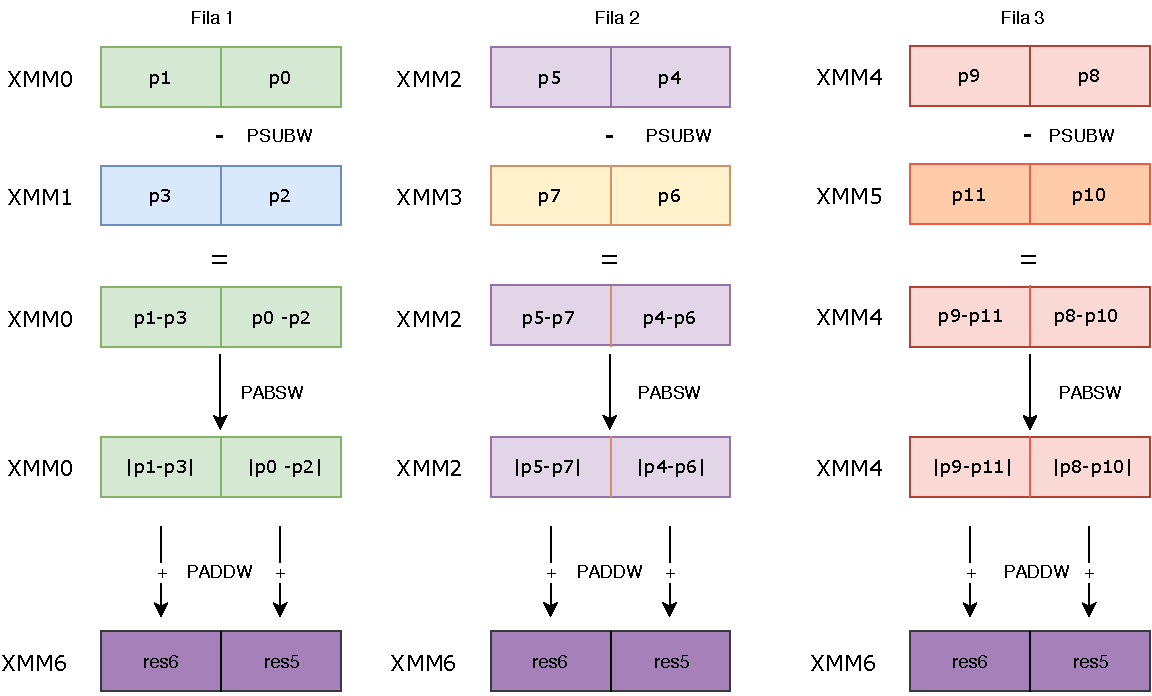
\includegraphics[scale=0.6]{img/sumHorizontalColorBordes.pdf}
		\caption{Suma de diferencias horizontales}
	\end{figure}

	Para calcular las diferencias verticales, se restan los registros correspondientes al mismo par de columnas, se toma valor absoluto y se suman a \textit{xmm6}. En este caso, las diferencias verticales de las columnas 2 y 3 deben ser sumadas tanto a la parte alta como a la parte baja del registro \textit{xmm6}, por lo que es necesario reordenar los resultados para sumar los valores que faltan. \\
	El siguiente esquema muestra gráficamente la operatoria realizada para obtener las sumas de las diferencias verticales:
	
	\begin{figure}[h]
		\centering
		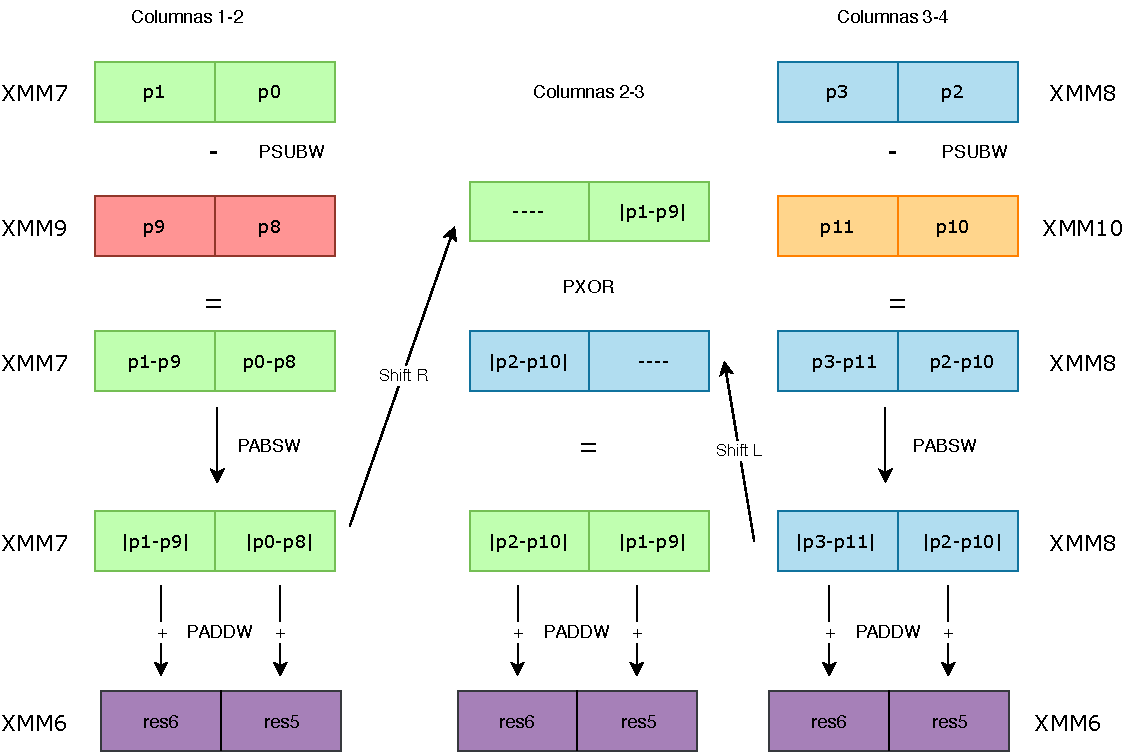
\includegraphics[scale=0.6]{img/sumVerticalesColorBordes.pdf}
		\caption{Suma de diferencias verticales}
	\end{figure}
	   
	Luego de acumular en \textit{xmm6} las sumas de las diferencias horizontales y verticales, se empaqueta el registro para convertir devuelta a byte y se arreglan las transparencias usando las máscaras destinadas a esto. Hecho esto, se mueven los resultados de los dos píxeles procesados a la imagen Destino y se actualizan los índices sumando 8 bytes a rdi y a rsi.
	
	Antes de avanzar de fila, se pinta de blanco el último píxel de la imagen Destino, de esta manera se arma el margen vertical derecho de la misma.
	\item \textbf{.bordesUltimaFila}\\
	Este ciclo realiza la misma operatoria que .bordesPrimeraFila, pero usa como registro contador a \textbf{r10d} y como registro índice a \textbf{edx}, que terminó con el valor 0 luego del primer ciclo bordes.
\end{itemize}
	
   
\subsubsection{Reforzar Brillo}

\justify
Nuevamente se definieron en primer lugar las máscaras a utilizar en la operatoria con los píxeles, estas son:
\begin{itemize}
	\item \textit{transparencia}: máscara utilizada para filtrar la componente de transparencia del píxel, la misma fue luego restaurada al terminar el ciclo usando la máscara \textit{fix}.
	\item \textit{green}: máscara utilizada para extraer la componente G del píxel, ya que es la única componente que duplica su valor al calcularse el brillo.
	\item \textit{fix}: máscara utilizada para fijar el valor de las transparencias de los píxeles al valor de 255.
\end{itemize} 
\justify
Previo a comenzar el ciclo, dichas máscaras fueron guardadas en los registros \textit{xmm15, xmm14 y xmm9}, respectivamente. Además, se guardaron las variables UmbralSup, UmbralInf, BrilloSup y BrilloInf en los registros \textit{xmm13, xmm12, xmm11 y xmm10}, respectivamente. Se realizó el \textit{broadcasting} necesario en dichos registros y, en el caso de los brillos, se empaquetaron en 8 bits teniendo en cuenta que si el valor era mayor a 255 debía saturarse a ese valor.
\justify
La idea principal de este algoritmo es recorrer la imagen levantando de memoria 4 píxeles consecutivos en el registro \textit{xmm4} y, utilizando registros auxiliares, calcular el brillo de cada píxel y determinar a cuales píxeles se les debe sumar brillo.

\begin{figure}[h]
	\centering
	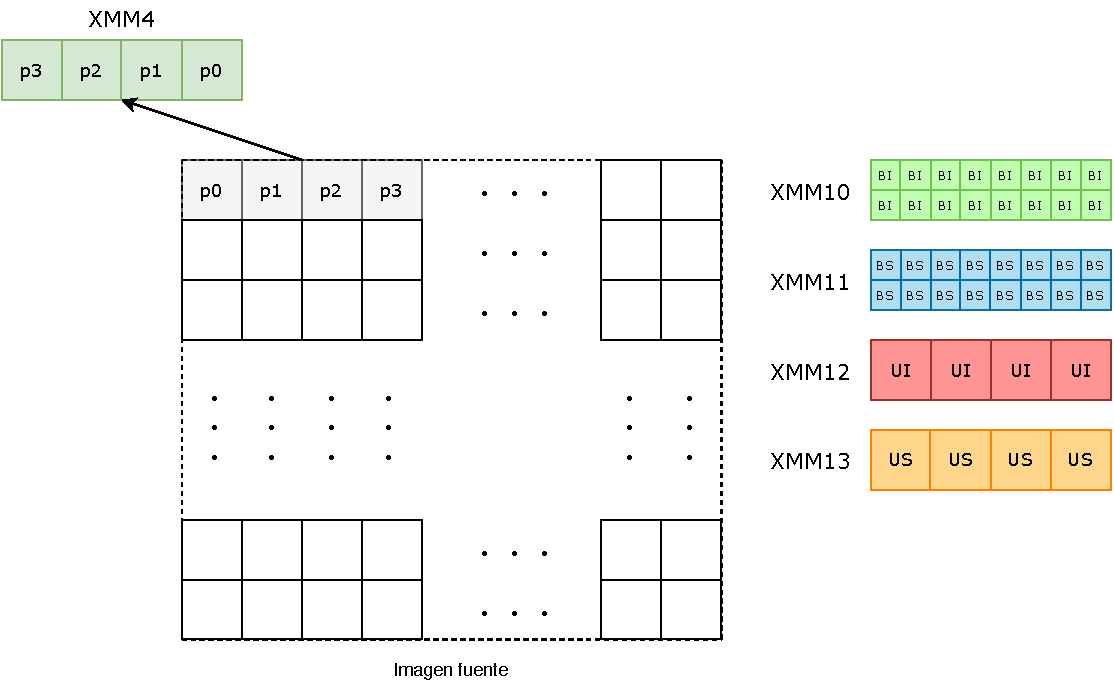
\includegraphics[scale=0.6]{img/LevReforzarBrillov2.pdf}
	\caption{Levantamiento de memoria Reforzar Brillo}
\end{figure}

\newpage 
\justify 
 Más específicamente, en cada iteración del ciclo se realizaron los siguientes pasos:
 
 \begin{enumerate}
 	\item \textbf{Cálculo de brillo}\\
 	Una vez levantados los 4 píxeles en el registro \textit{xmm4} se elimina la transparencia de estos utilizando la máscara \textit{transparencia} puesto que la componente A no es necesaria en el cálculo de brillo. Para efectuar los cálculos propicios, se realiza una copia de los valores de \textit{xmm4} en \textit{xmm3}. Posteriormente, se extraen al registro \textit{xmm2} las componentes G de cada píxel utilizando la máscara \textit{green} y se setean en cero en el registro \textit{xmm3}.\\
 	Para poder realizar el cálculo de brillo correctamente es necesario extender las componentes R, G y B de \textit{byte} a \textit{word} puesto que al realizar las operaciones requeridas los valores resultantes podrían excederse del rango numérico propio del \textit{byte}. Por este motivo las componentes G de los píxeles en \textit{xmm2} primero se alinean a \textit{word} y luego se multiplican por 2. Por otro lado, las componentes R y G, que se encuentran aún en \textit{xmm3}, están alineadas ya a \textit{word}, por lo que se procede a realizar la suma horizontal de estas dos con el formato de 16 \textit{bits}.\\
 	Por una cuestión de conveniencia, se desempaquetan las sumas de las componentes R y B de los 4 píxeles que se encuentran en la parte baja de \textit{xmm3}, transformándolas de \textit{word} a \textit{dword}.  Gracias a que los valores de 2*G  en \textit{xmm2} están alineados a \textit{dword}, se procede a sumar los valores correspondientes a cada píxel en el formato de 32 \textit{bits}. De esta manera se obtiene en el registro \textit{xmm3} los brillos correspondientes a cada pixel pero multiplicados por 4. Simplemente shifteando a derecha dos veces cada \textit{dword} se obtienen finalmente los 4 brillos definidos en la operación: 
 	 \begin{equation}
 	B = (src[i][j].r + 2 * src[i][j].g + src[i][j].b)/4 
 	\end{equation}
 	 
\begin{figure}[h!]
	\centering
 	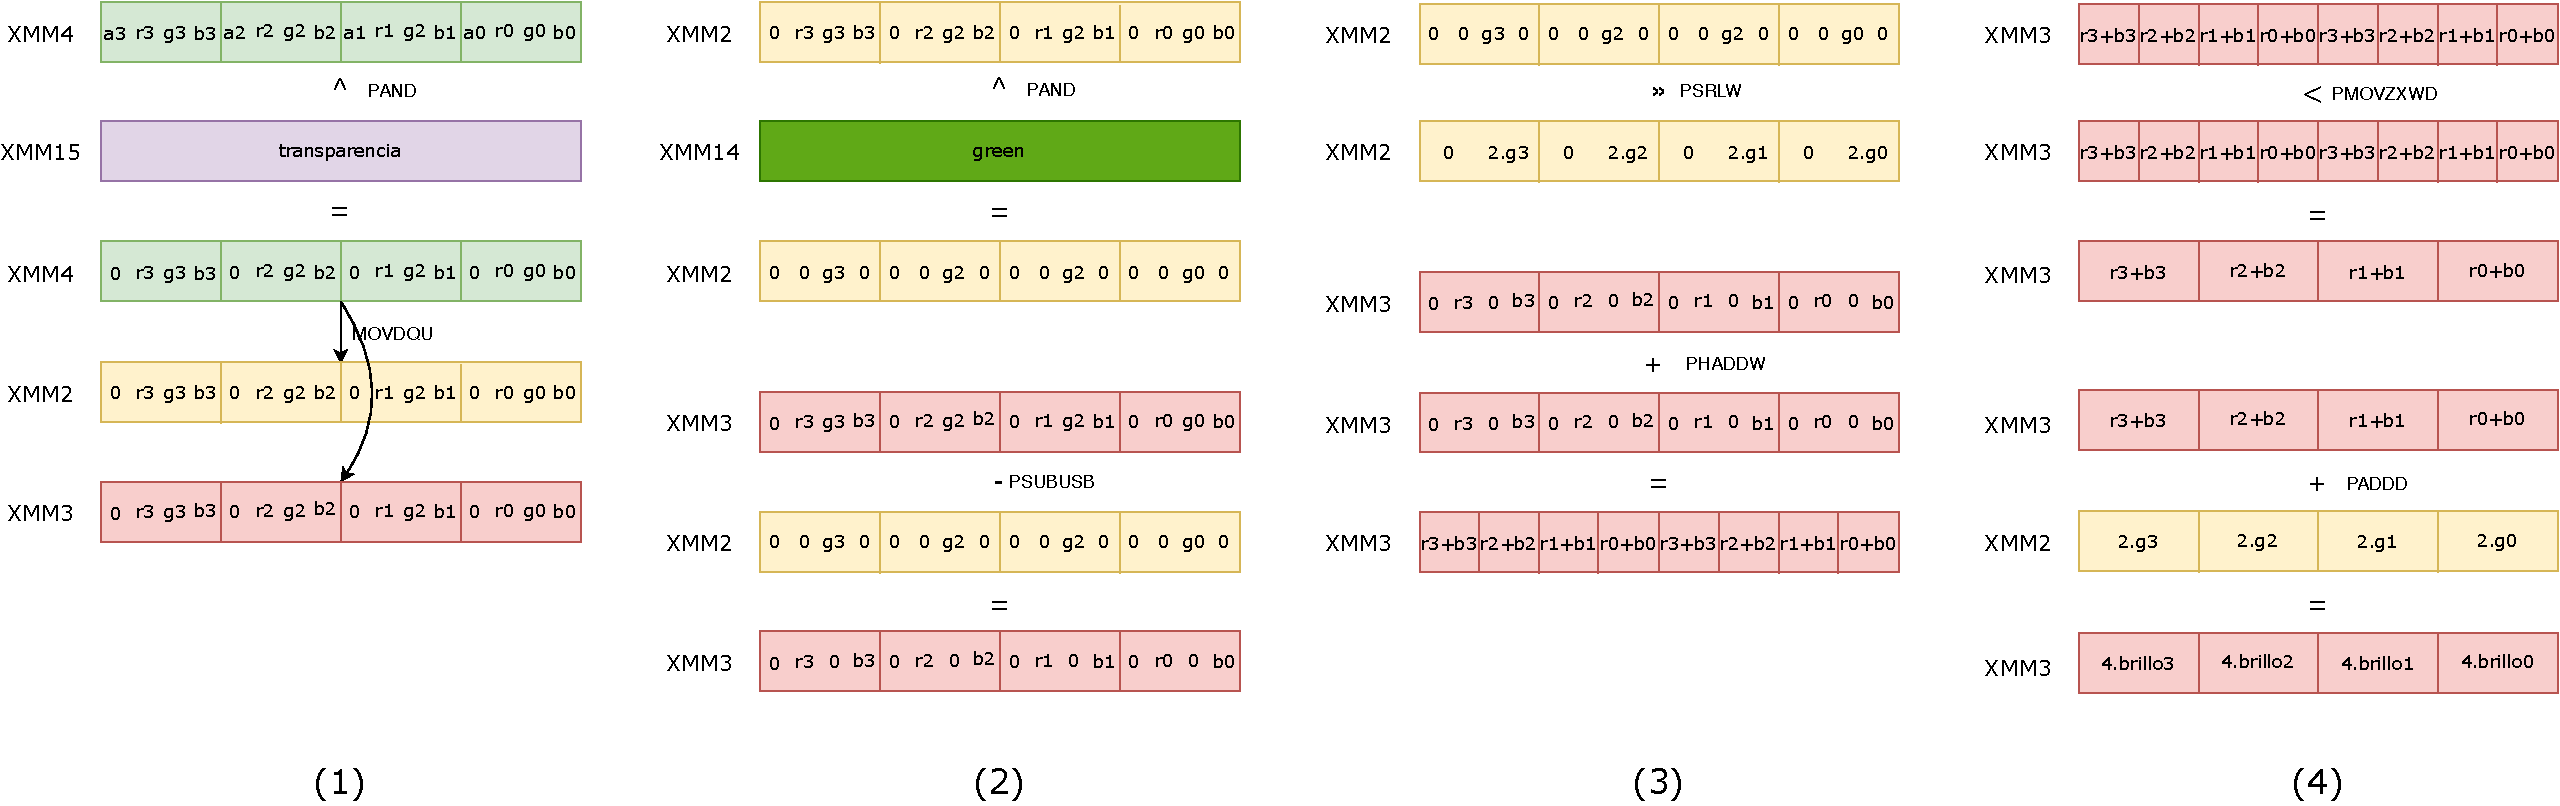
\includegraphics[scale=0.35]{img/ReforzarBrillo2.pdf}
 	\caption{Cálculo de brillo}
 \end{figure}
 
 	\item \textbf{Adición de brillo superior}\\
 	
	Una vez calculados los 4 brillos se mueven al registro \textit{xmm6}, donde luego son comparados uno a uno con los valores de umbral superior, guardados en \textit{xmm13}. En caso de que un brillo sea mayor al umbral superior, se guarda en \textit{xmm6} en los 32 \textit{bits} correspondientes una máscara con 1s. Caso contrario, se guarda en esa posición una máscara con 0s. Con ayuda de estas máscaras y utilizando los valores guardados en \textit{xmm11} se colocan en \textit{xmm6} 4 brillos superiores en los 32 \textit{bits} donde correspondan. Finalmente se suman \textit{byte} a \textit{byte} los registros \textit{xmm4} y \textit{xmm6}, de forma saturada.
 	
 	\item \textbf{Substracción de brillo inferior}\\
 	
 	Para realizar la substracción del brillo inferior, se transfieren ahora a \textit{xmm6} los umbrales inferiores guardados en \textit{xmm12} para que luego sean comparados uno a uno con los brillos de cada píxel. De manera análoga a la anterior, en caso de que un umbral inferior sea mayor al brillo se guarda en esa posición una máscara con 1s, y en el caso contrario con 0s. Nuevamente con ayuda de estas máscaras y ahora utilizando los valores de brillo inferior guardados en \textit{xmm13} se colocan en \textit{xmm6} 4 brillos inferiores en los 32 \textit{bits} donde correspondan. Luego se restan \textit{byte} a \textit{byte} los registros \textit{xmm4} y \textit{xmm6}, de forma saturada.
 	
 	En último lugar se arreglan las transparencias de los píxeles con la máscara \textit{fix} y se cargan los 4 pixeles a la imagen Destino.
 	
 	\begin{figure}[h]
 		\centering
 		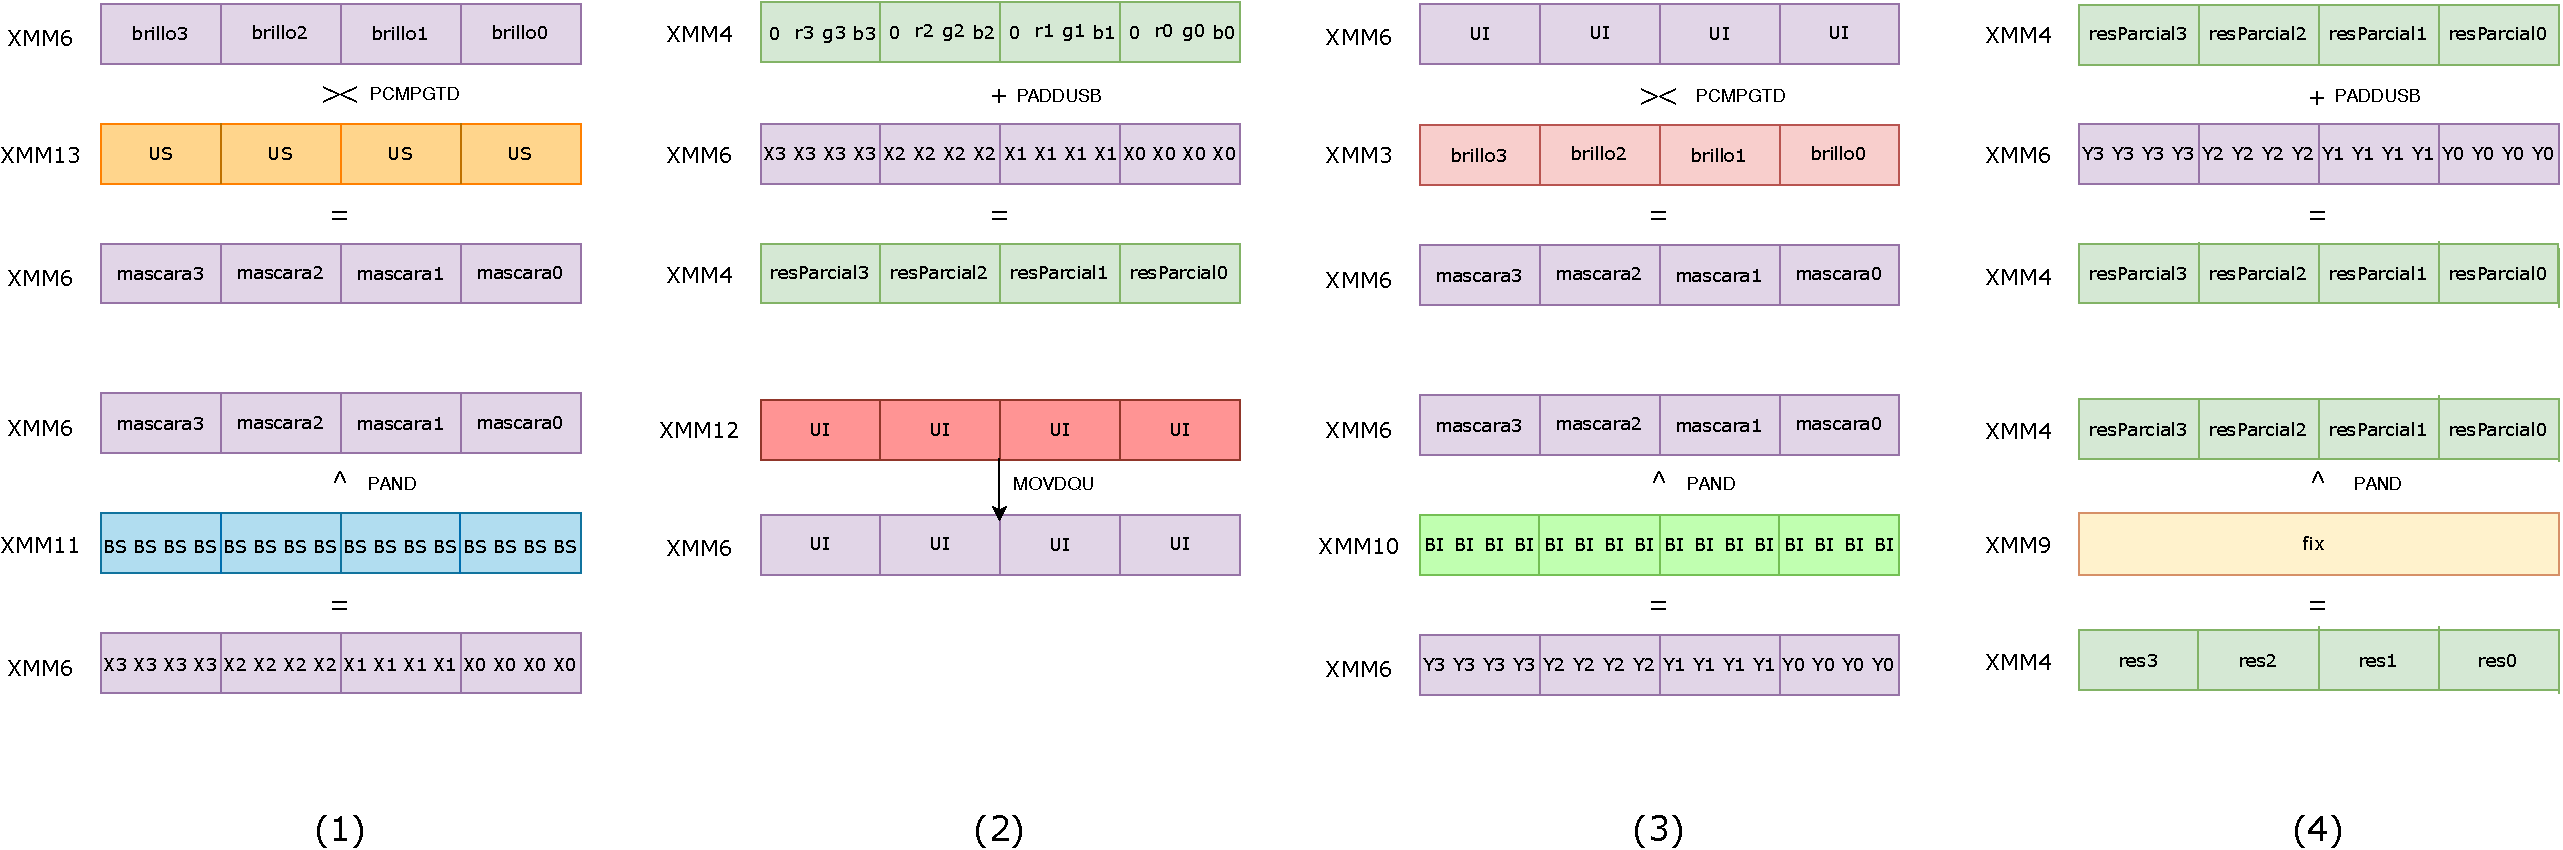
\includegraphics[scale = 0.37]{img/ReforzarBrillo3.pdf}
 		\caption{Adición de brillo superior y brillo inferior}
 	\end{figure}
 	
 	    
 \end{enumerate}


\subsection{Comparación entre implementaciones en ASM y C}
\subsubsection{Objetivo}
\justify
El propósito de esta sección es comparar cada una de las implementaciones de los filtros codificadas en lenguaje ensamblador contra las implementaciones en C, provistas por la cátedra. La comparación realizada está centrada en el rendimiento de las implementaciones en ambos lenguajes, en función de los tamaños de las imágenes. Para el caso de las implementaciones en C, se compara el rendimiento utilizando las distintas opciones de optimización del código. 
\justify
La forma de medir el rendimiento se realizó mediante la toma de tiempos de ejecución, utilizando el \textit{Time Stamp Counter (TSC)}, registro del procesador que cuenta el número de ciclos del mismo y permite así calcular la cantidad de ciclos de ejecución de un filtro, a partir de la diferencia entre los contadores previos y posteriores a la llamada de la función del mismo. 
\justify
Dado que el registro TSC se ve afectado por diversos factores (\textit{scheduling}, estado del procesador, etc), el tiempo de ejecución medido no siempre es el mismo, ni es exacto, por lo que fue necesario definir un protocolo de toma de mediciones, con el objetivo de reducir el \textit{ruido} que producen esos factores en la medición y poder obtener una muestra representativa del tiempo de ejecución. El mismo consistió en reducir al mínimo la cantidad de programas ejecutándose al momento de tomar las mediciones, y tomar muestras con gran cantidad de datos (200 repeticiones), a las que luego se les eliminaron los \textit{outliers}.
\justify

\subsubsection{Metodología}
\justify
Las mediciones fueron tomadas en una computadora con las siguientes especificaciones: procesador Ryzen 5 3600 y RAM de 2x8gb Corsair corriendo a 3200mhz.

\justify
Para la comparación de rendimiento a un tamaño fijo de imagen (1280x720), se tomaron 5 muestras de 200 datos para cada filtro (Imagen Fantasma, Color Bordes y Reforzar Brillo), correspondientes a la implementación en ASM y a la implementación en C, compilada con GCC bajo los siguientes casos:
\begin{enumerate}
	\item Caso 1: Implementación en C usando la optimización del compilador \textbf{-O0}.
	\item Caso 2: Implementación en C usando la optimización del compilador \textbf{-O1}.
	\item Caso 3: Implementación en C usando la optimización del compilador \textbf{-O2}.
	\item Caso 4: Implementación en C usando la optimización del compilador \textbf{-O3}.
\end{enumerate}

\justify
Para la comparación de rendimiento en función del tamaño de las imágenes, se tomaron 7 muestras de 200 datos para las implementaciones de ASM y de C-O3(que se hipotetiza que es la más eficiente), de los siguientes tamaños:
\begin{enumerate}
	\item  Tamaño de imagen 1: 32x16
	\item  Tamaño de imagen 2: 64x32
	\item  Tamaño de imagen 3: 128x64
	\item  Tamaño de imagen 4: 256x128  
	\item  Tamaño de imagen 5: 512x256
	\item  Tamaño de imagen 6: 1024x512
	\item  Tamaño de imagen 7: 2048x1024
\end{enumerate}

\justify	
Para eliminar los \textit{outliers}, a cada muestra se le calculó su media alfa-podada a ambos extremos, eliminando 40 valores. De esta manera se obtuvieron muestras más representativas del "valor real" \ del tiempo de ejecución de cada implementación.

\justify 
Además, se calculó el desvío estándar de cada muestra, para obtener un valor que sirva para comparar la dispersión de los datos. Con los datos de la media y del desvío estándar se confeccionaron tablas que se encuentran en el anexo.

\justify 
Finalmente, a partir de las mediciones se confeccionaron gráficos para condensar la información obtenida en la toma de datos.\\

\justify 
\subsubsection{Resultados}

\justify 
A continuación se presentan los resultados de la comparación de las implementaciones en ASM, C con optimización -O0, C con optimización -O1, C con optimización -O2 y C con optimización -O3, para todos los filtros.
\justify 
Seguidamente, se presentan los resultados de la comparación de rendimiento en función de los tamaños de las imágenes, para ASM y C con optimización -O3.\\ 

\begin{figure}[h!]
	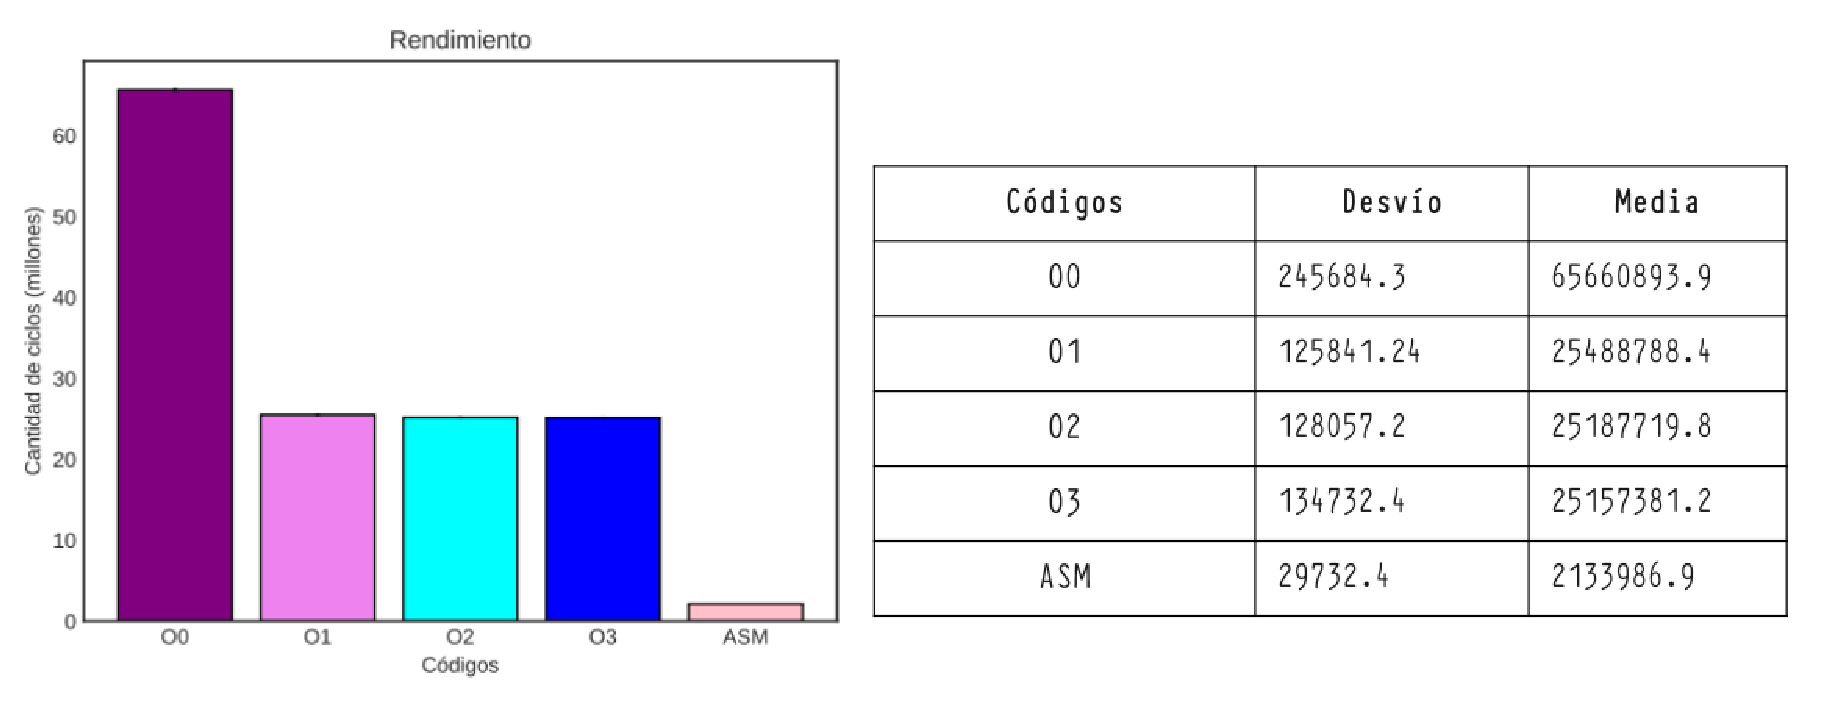
\includegraphics[scale=0.55]{img/ImagenFantasmaConTabla.pdf}
	\caption{Gráfico de barras de rendimiento de las implementaciones de Imagen Fantasma.}
\end{figure}	



\begin{figure}[h!]
	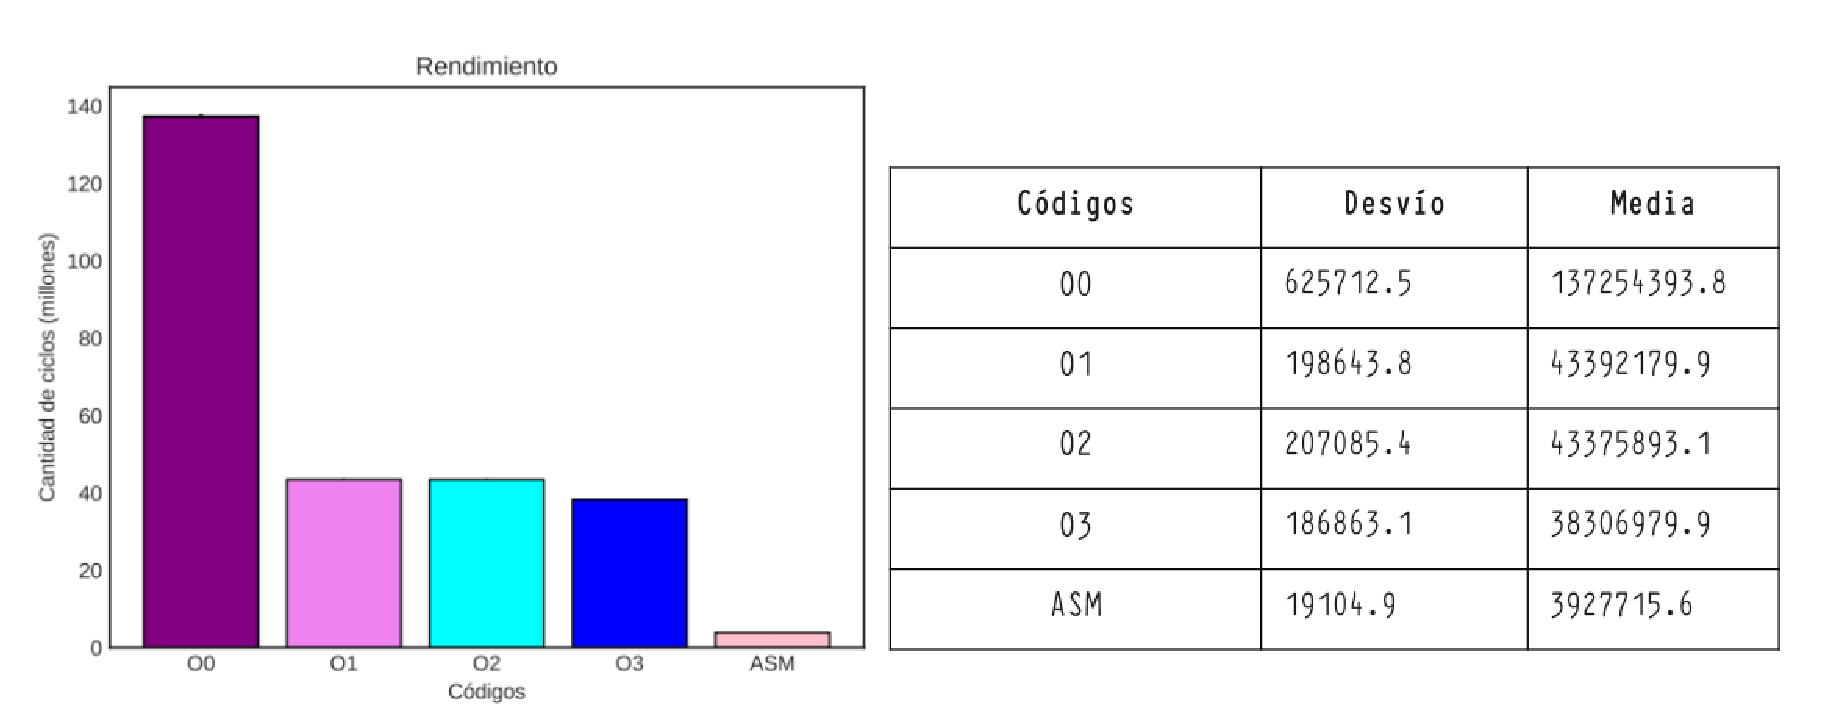
\includegraphics[scale=0.55]{img/ColorBordesConTabla.pdf}
	\caption{Gráfico de barras de rendimiento de las implementaciones de Color Bordes.}
\end{figure}	


\begin{figure}[h!]
	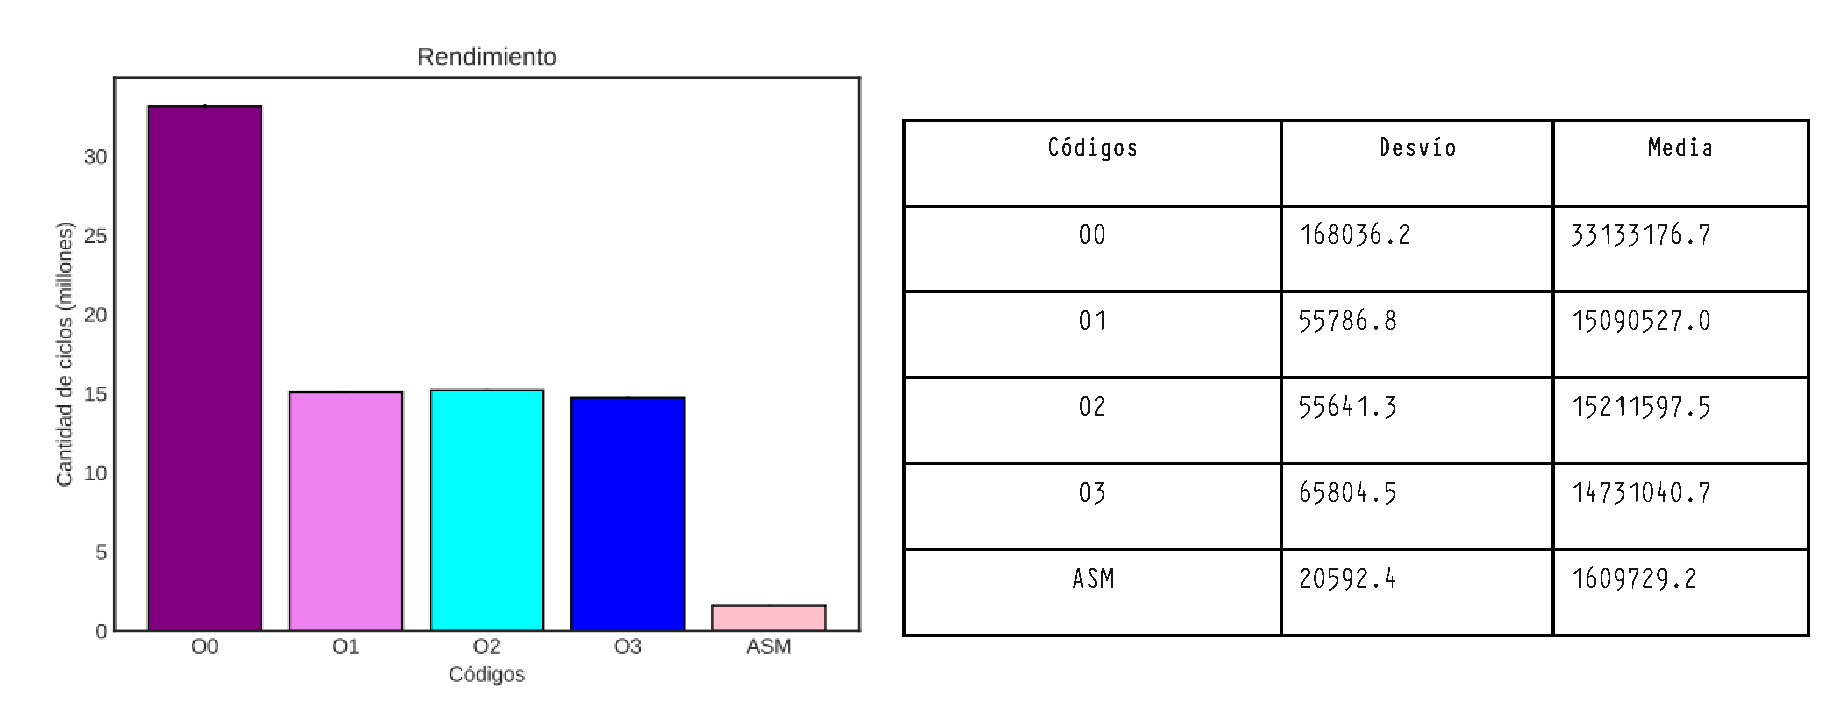
\includegraphics[scale=0.55]{img/ReforzarBrilloConTabla.pdf}
	\caption{Gráfico de barras de rendimiento de las implementaciones de Reforzar Brillo.}
\end{figure}



\begin{figure}[h!]
	\centering
	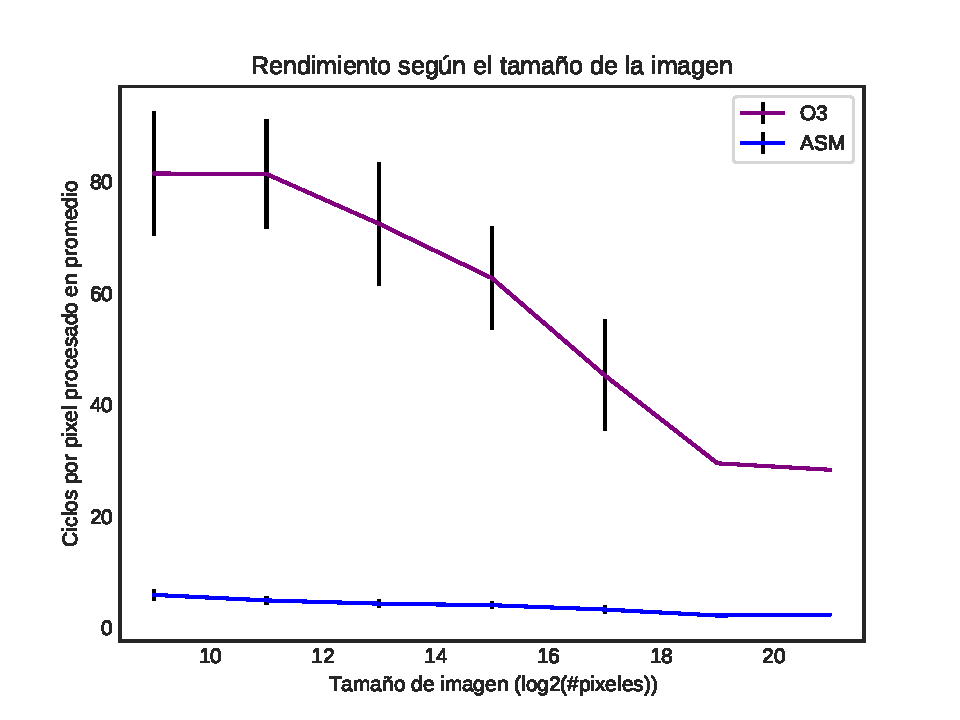
\includegraphics[scale=0.56]{img/ImagenFantasmaO3vsASM.pdf}
	\caption{Comparación de rendimiento en función del tamaño del filtro Imagen Fantasma}
\end{figure}	


\begin{figure}[h!]
	\centering
	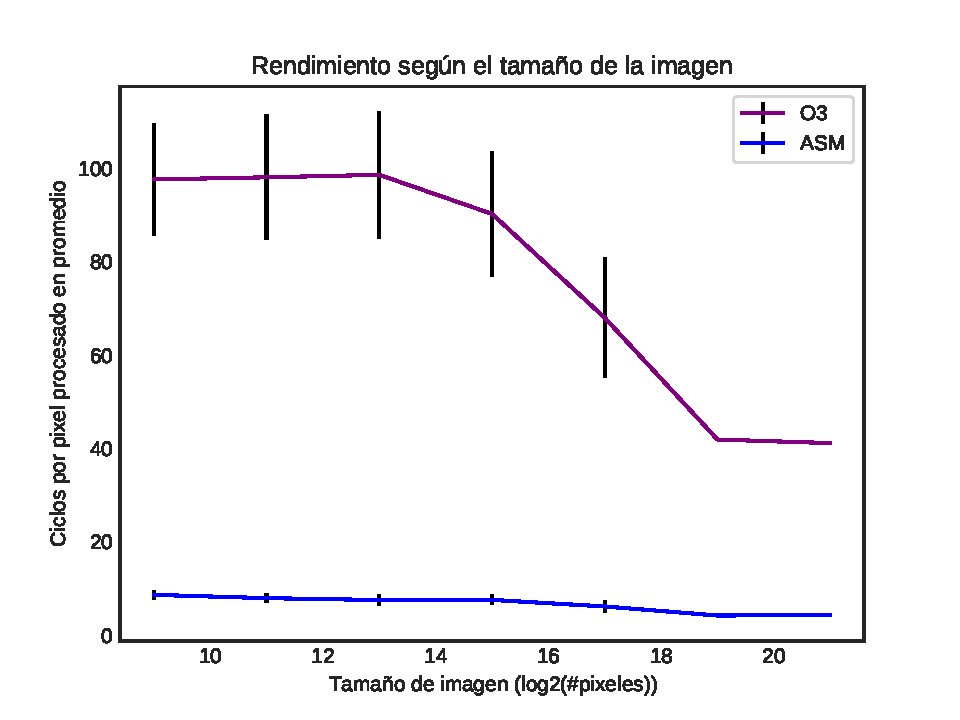
\includegraphics[scale=0.56]{img/ColorBordesO3vsASM.pdf}
	\caption{Comparación de rendimiento en función del tamaño del filtro Color Bordes}
\end{figure}	


\begin{figure}[h!]
	\centering
	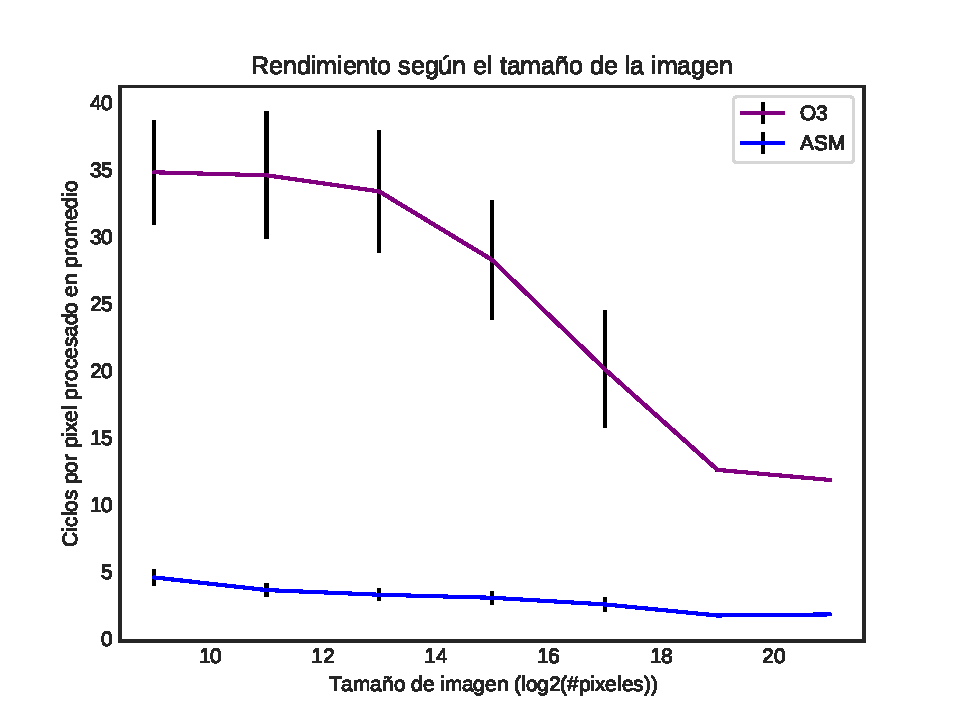
\includegraphics[scale=0.56]{img/ReforzarBrilloO3vsASM.pdf}
	\caption{Comparación de rendimiento en función del tamaño del filtro Reforzar Brillo}
\end{figure}


\subsubsection{Conclusiones}
\justify 
En un primer lugar, a partir de los resultados de la comparación de rendimiento entre ASM y C, se puede concluir a simple vista que el rendimiento de la implementación en ASM es mucho mayor que el rendimiento de C, sin importar la optimización del código. En todos los casos, el tiempo de ejecución de la implementación en ASM es menor al 10\% del tiempo de ejecución de la implementación en C. Dentro de las distintas optimizaciones de C, se percibe una notable diferencia entre la optimización O0 y el resto, siendo esta la menos eficiente de las cuatro. Dentro de las tres optimizaciones restantes (O1, O2 y O3), no se observan diferencias significativas en ninguno de los tres filtros, aunque sí puede remarcarse una leve diferencia entre O2 y O3 en el filtro de \textit{<<Color Bordes>>}.
\justify 
Por otro lado, en el caso de la comparación de rendimiento en función del tamaño, nuevamente se observa una gran diferencia de rendimiento entre ambos lenguajes. En este caso, el porcentaje que equivale el tiempo de ejecución de ASM con respecto a C-O3, para las imágenes de mayor tamaño, es de 8.4\%, 10\%, 15\%, para los filtros Imagen Fantasma, Color Bordes y Reforzar Brillo , respectivamente, concluyéndose con mayor seguridad, gracias al bajo desvió estándar, que la implementación en ASM es la mejor. Para todos los casos la gráfica es similar: la curva de C es una función decreciente que se estanca a partir del tamaño de 1024x512 píxeles y la curva de ASM es una función levemente decreciente que también se estanca en los mismos valores. En cuanto a las barras de error, se percibe una gran diferencia de tamaño de las mismas en la curva de ASM respecto a la de C. Se cree que esto podría deberse a que la implementación de C posee más \textit{ruido}, por tener un tiempo de ejecución mucho mayor. A su vez, a partir del valor en que las curvas se estancan, las barras de error ya no son distinguibles en el gráfico, esto podría deberse a que a un tamaño grande de imagen el ruido ya no es significativo. De todas formas, los resultados no son suficientes para obtener una conclusión con respecto a este tema.
\justify En conclusión, la implementación en lenguaje ensamblador es mucho más eficiente que la implementacion en C, sin importar la optimización usada. Además, la implementación en C parece mejorar a tamaños mayores de imagenes, aunque sigue sin alcanzar a ASM.

     
\subsection{Diseño experimental}

\subsubsection{Experimento 1: Int vs Float para el filtro Imagen Fantasma}

\justify
\textbf{Objetivos e hipótesis}
\justify
El siguiente experimento está inspirado en las siguientes preguntas:
\justify
\begin{enumerate}
	\item \textit{¿Hay diferencias entre operar con enteros o punto flotante? ¿La imagen final tiene diferencias significativas?}
	\item \textit{¿Cuál implementación es “mejor”?}
	\item \textit{¿Existe alguna relación de ganancia en rendimiento a cambio de pérdida de precisión?}
\end{enumerate}

\justify
Durante el desarrollo de este trabajo práctico se realizaron dos implementaciones distintas para el filtro de \textit{<<Imagen Fantasma>>}: una que procesa los datos como enteros, detallada anteriormente en la sección \textit{2.1.1}, y otra que procesa los datos como números flotantes de 32 bits (precisión simple). La implementación con \textit{int} levanta cuatro pixeles en dos accesos a memoria y procesa simultáneamente dos píxeles, mientras que la otra implementación levanta cuatro pixeles en cuatro accesos a memoria, y no procesa ninguno de manera simultánea. La idea de este experimento es comparar el rendimiento y la pérdida de precisión (si es que la hay) de ambas implementaciones y formular una relación entre ambas, poniendo a prueba la siguiente hipótesis:

\justify
\textit{Para un mismo tamaño de imagen, el rendimiento de la implementación en enteros será mayor que el de la implementación en números flotantes, dado que procesa más píxeles en simúltaneo y realiza menos accesos a memoria. Para las imágenes con mayor cantidad de píxeles con brillo alto, se perderá menos precisión ya que estos se saturarán. Asimismo, para las imágenes con mayor cantidad de píxeles con brillo bajo, se perderá precisión, pero está pérdida será de a lo sumo una unidad por componente en la mayoría de los casos. En cambio, en las imágenes de brillo medio, la pérdida será mayor que las anteriores. Sin embargo, esta pérdida de precisión no será significativa en relación al aumento del rendimiento, en ninguno de los casos.}   
\begin{figure}[h]
	\centering
	\begin{subfigure}[b]{0.3 \textwidth}
		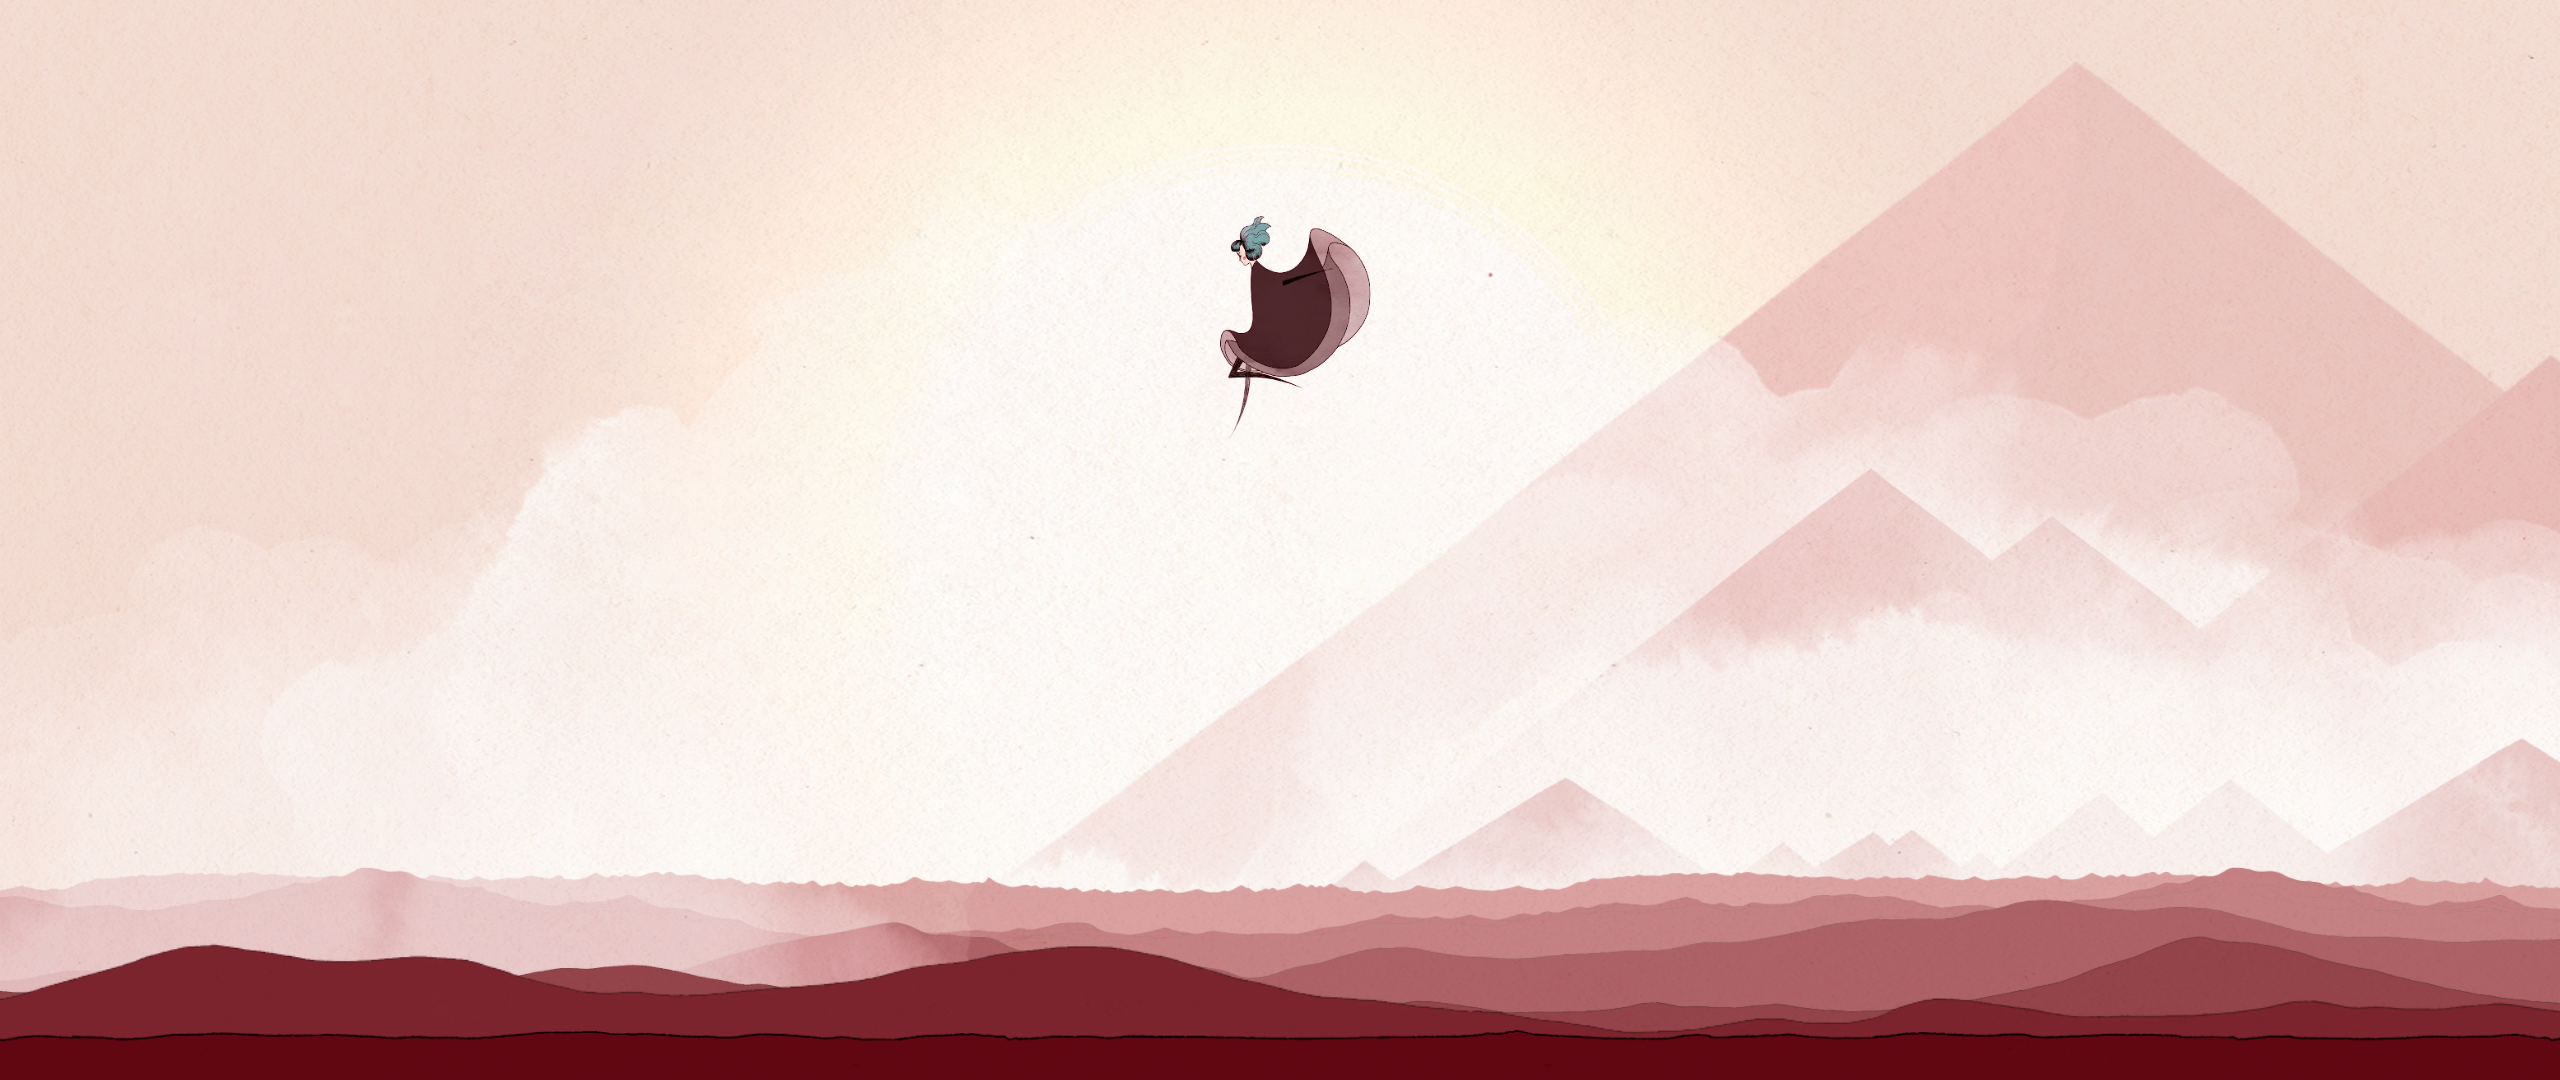
\includegraphics[width=\textwidth]{img/bajo1.png}
		\caption{Imagen con brillo alto}
	\end{subfigure}
	\hfill
	\begin{subfigure}[b]{0.3 \textwidth}
		
\includegraphics[width=\textwidth]{img/gris5.jpg}
		\caption{Imagen con brillo medio}
	\end{subfigure}
	\hfill
	\begin{subfigure}[b]{0.3 \textwidth}
		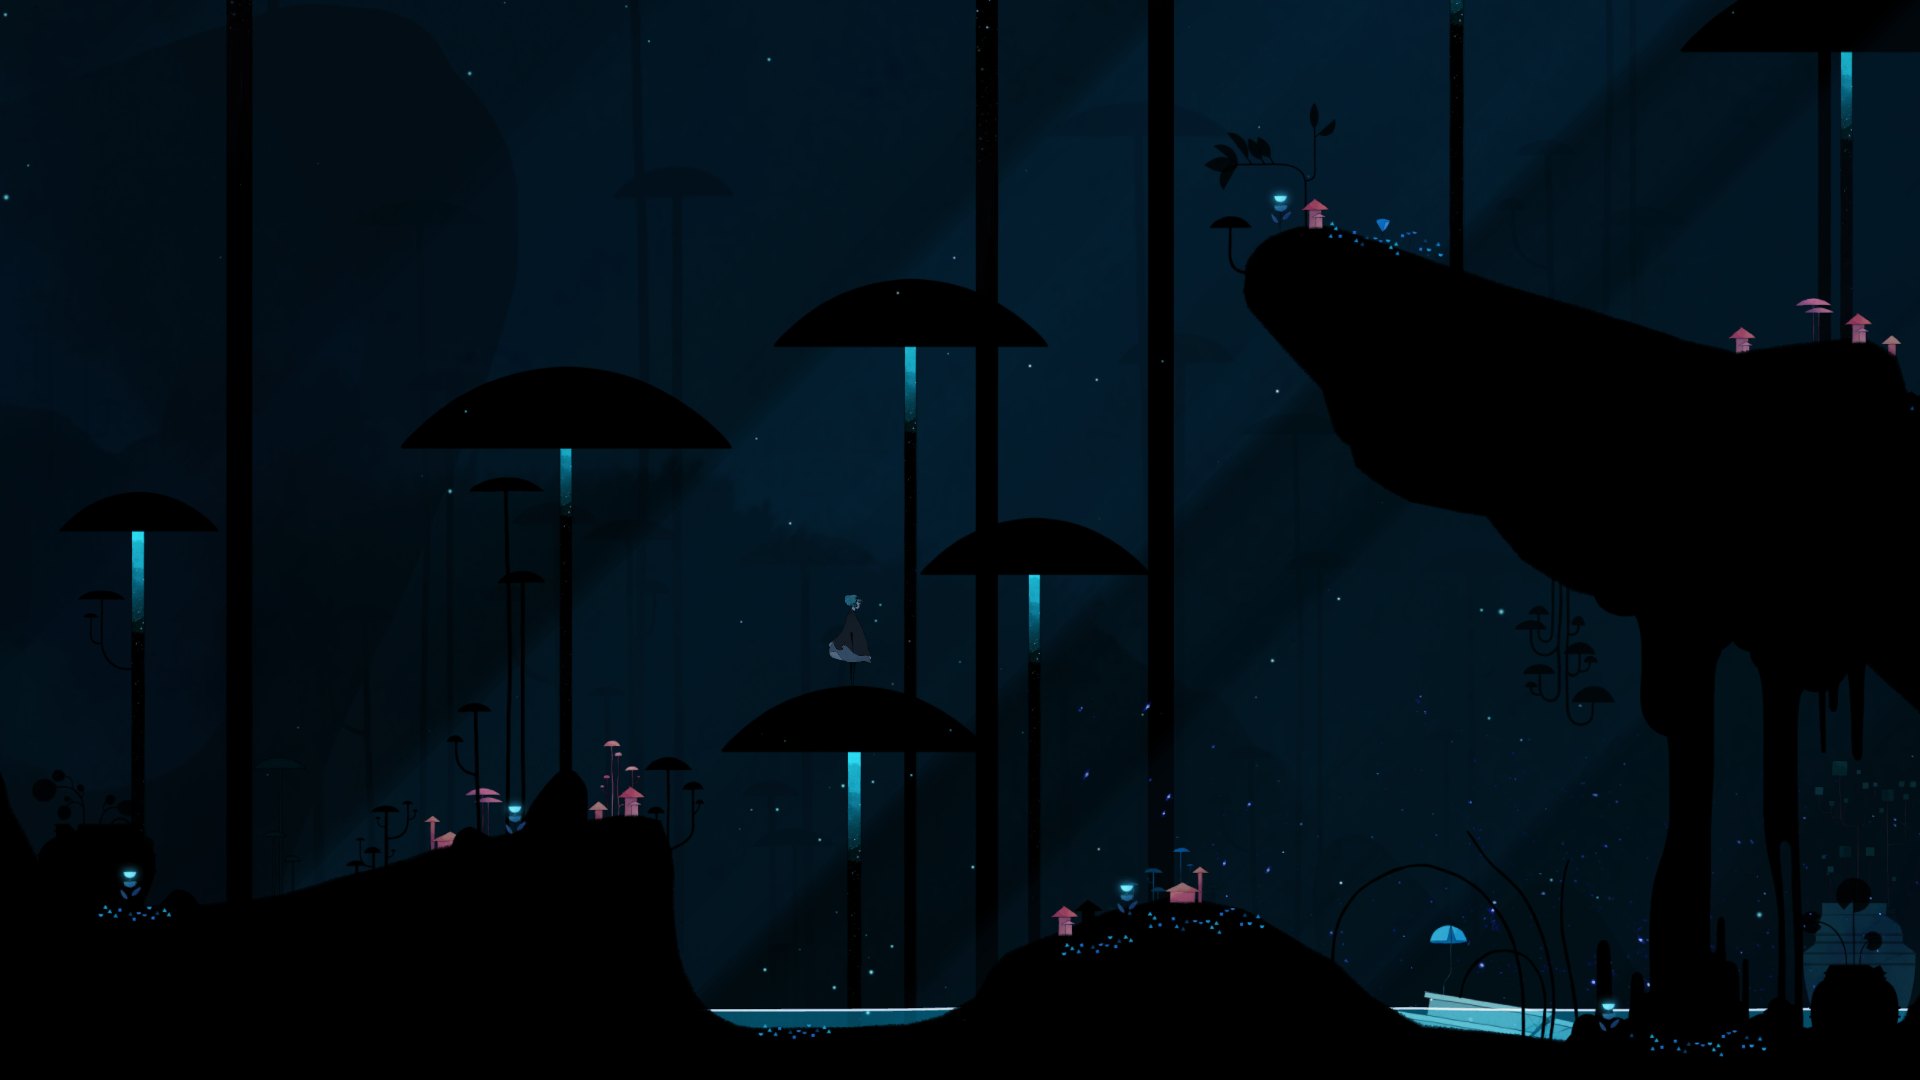
\includegraphics[width=\textwidth]{img/oscura2.png}
		\caption{Imagen con brillo bajo}
	\end{subfigure}
	\caption{Imagenes utilizadas para el experimento}
\end{figure}

\newpage
\justify
\textbf{Metodología}
\justify
Se seleccionaron tres imagenes segun sus tonalidades y tipos de brillo, con el objetivo de poder comparar la pérdida de precisión dependiendo de la cantidad de brillo de la imagen. 
\justify
Las imagenes seleccionadas tienen las siguientes características:
\begin{enumerate}
	\item Imagen 1: Mayoría de pixeles con brillo bajo, tonos azulados y negros.
	\item Imagen 2: Mayoría de píxeles con brillo medio, tonos violetas y celestes.
	\item Imagen 3: Mayoría de píxeles con brillo alto, tonos claros. 
\end{enumerate}
\justify
Antes de comenzar con los experimentos, se convirtió el formato de las imagenes a .bmp y se cambió el tamaño de las imagenes a 1280x720, para poder hacer una mejor comparación.
\justify
Para comparar el rendimiento, se realizó el mismo procedimiento que en la comparación de C vs ASM, en este caso tomando 3 muestras de 200 valores cada una, correspondientes a cada caso de brillo, para ambas implementaciones del filtro \textit{<<Imagen Fantasma>>}. 
\justify
En la comparación de precisión se utilizó el \textit{bmpdiff}. Para cada caso de brillo se generó una imagen con el filtro \textit{<<Imagen Fantasma>>}  y una imagen utilizando la implemetación en C de la cátedra. Luego, se comparó cada imagen usando el \textit{bmpdiff} contando la cantidad de componentes que diferían en a lo sumo 2 unidades de la implementación en C. El valor obtenido hace referencia a la cantidad de componentes que pierden precisión.
\justify
Realizando este método se registraron la cantidad de componentes que 
no pierden precisión, que pierden una unidad de precisión y que pierden dos unidades de precisión, para cada caso.

\subsubsection{Experimento 2: Rendimiento en función de la cantidad de accesos a memoria y píxeles procesados para el filtro Reforzar Brillo}

\justify
\textbf{Objetivos e hipótesis}
\justify
Este experimento está inspirado en las siguientes preguntas:
\justify
\begin{enumerate}
	\item \textit{¿Cuál es la cantidad de pixeles procesados en cada implementación? ¿Y de accesos a memoria? ¿Se condice empíricamente esta diferencia en la performance de los filtros?}
	\item \textit{¿Cuál implementación es “mejor”?}	 
\end{enumerate}
\justify
El objetivo detrás de este experimento es evaluar el rendimiento en función de la cantidad de píxeles procesados y accesos a memoria, utilizando dos implementaciones realizadas para el filtro de \textit{<<Reforzar Brillo>>} que difieren en estas dos métricas. La primera implementación levanta y procesa dos píxeles en simultáneo, mientras que la segunda implementación levanta y procesa cuatro píxeles, también en simultáneo. El experimento realizado busca poner a prueba la siguiente hipótesis:
\justify
\textit{La implementación que realiza menor cantidad de accesos a memoria y procesa mayor cantidad de píxeles en simultáneo es la más eficiente en términos de tiempo de ejecución. El rendimiento de la segunda implementación(cuatro píxeles en simultáneo) será de al menos el doble que el rendimiento de la primera(dos píxeles en simultáneo). }

\justify
\textbf{Metodología}
\justify
Se realizó una comparación de rendimiento similar a la realizada en el los experimentos anteriores, aplicando las implementaciones del filtro \textit{<<Reforzar Brillo>>} a la imagen \textit{<<SweetNovember>>} con los siguientes tamaños: [32x16, 64x32, 128x64, 256x128, 512x256, 1024x512, 2048x1024, 4096x2048]. Para cada tamaño de imagen se tomaron los datos con ambas implementaciones, siguiendo el mismo protocolo de toma de mediciones y eliminación de \textit{outliers} que se detalló en las secciones anteriores.




\section{Resultados}
\subsection{Experimento 1}

\justify
Los gráficos presentados a continuación reflejan los resultados de la comparación de pérdida de precisión entre las tres imagenes utilizadas, para el algoritmo de \textit{<<Imagen Fantasma>>} que realiza las operaciones con números enteros. En cuanto a la implementación en floats, no se observó pérdida de precisión para ninguno de los tres casos de brillo.
 
\begin{figure}[h]
	\centering
	\begin{subfigure}{0.49 \textwidth}
		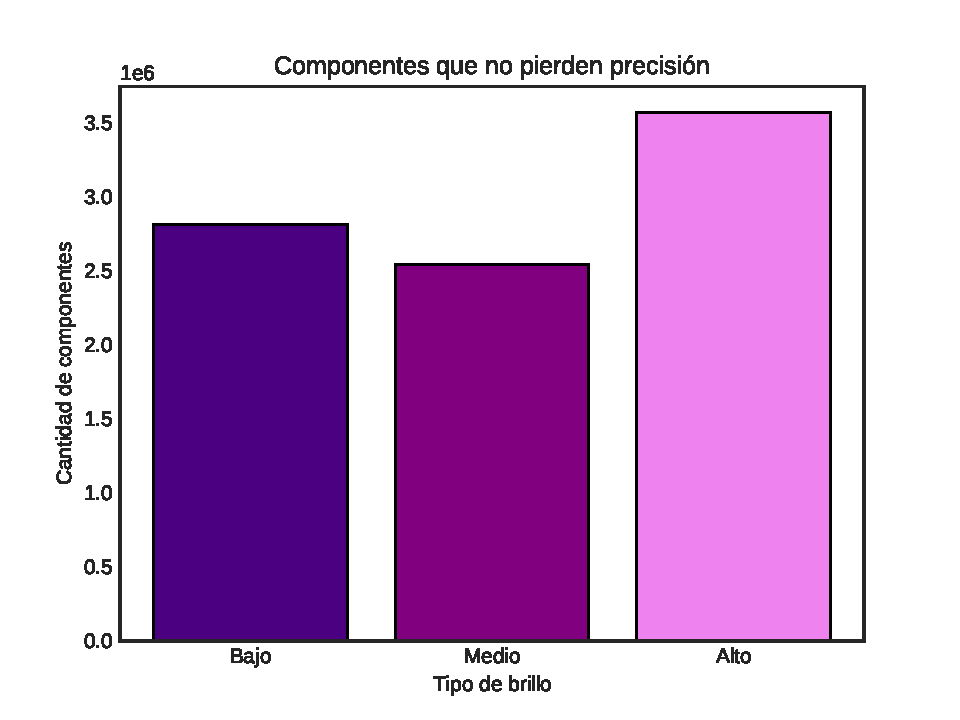
\includegraphics[width=\textwidth]{img/Precision0.pdf}
			\caption{Comparación de cantidad de componentes que no pierden precisión}
	\end{subfigure}
	\hfill
	\begin{subfigure}{0.49 \textwidth}
		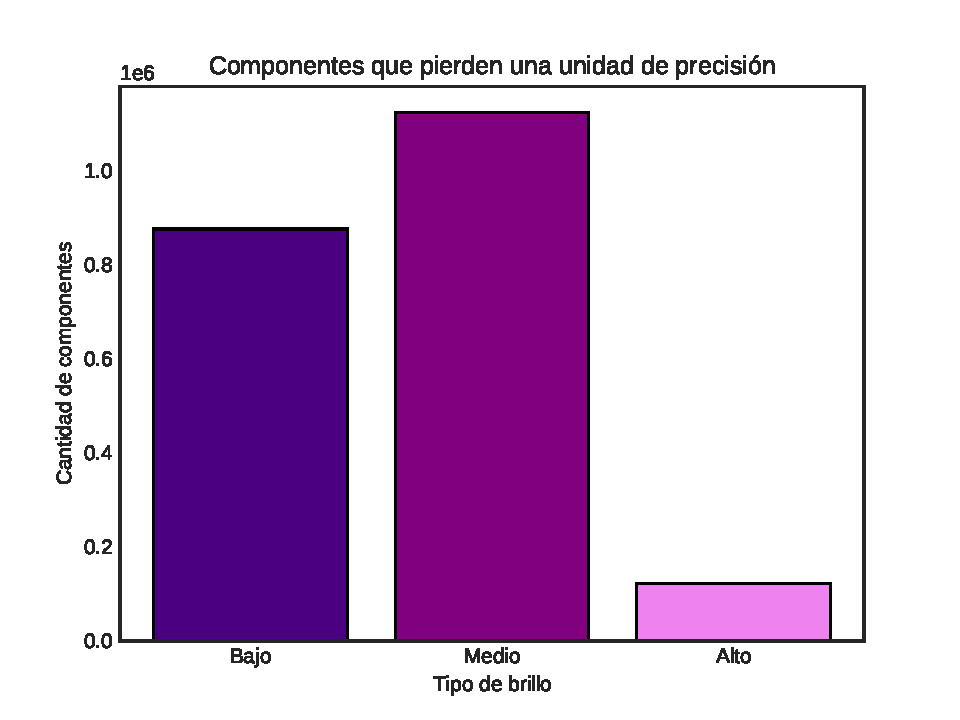
\includegraphics[width=\textwidth]{img/Precision1.pdf}
		\caption{Comparación de cantidad de componentes que pierden una unidad precisión}
	\end{subfigure}
	\centering
	\begin{subfigure}{0.49 \textwidth}
		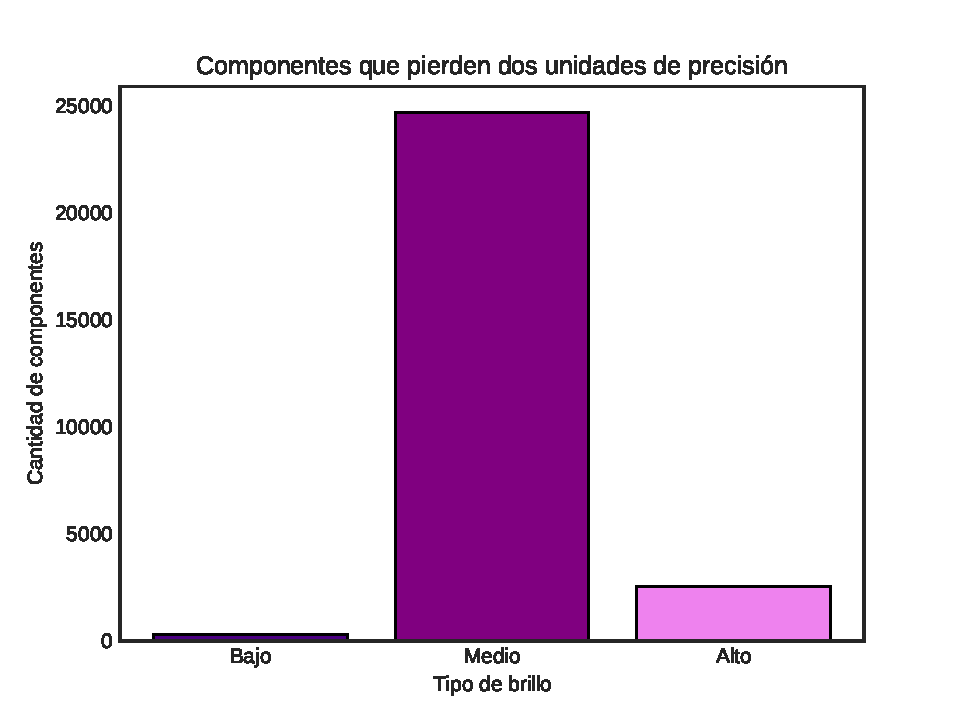
\includegraphics[width=\textwidth]{img/Precision2.pdf}
		\caption{Comparación de cantidad de componentes que pierden dos unidades precisión.}
	\end{subfigure}
	\caption{Graficos de barras de comparación int vs Float}
\end{figure}
\justify
Se observa una marcada diferencia entre los tres tipos de brillo para los casos de las componentes que pierden precisión. La pérdida de precisión por una unidad predomina en las imágenes de brillo bajo y medio, mientras que la pérdida de precisión por dos unidades predomina solo en las imágenes de brillo medio, siendo los valores mucho más pequeños que en el caso anterior.
\justify
Para el caso en el que las componentes mantienen la precisión, no se observan diferencias muy marcadas, pero sí se puede distinguir que las que menos pierden precisión pertenecen a la imagen de brillo alto, seguidas por las de brillo bajo. La pérdida de precisión por píxel en promedio de los tres tipos de brillos es de: 0.23, 0.31, 0.03 para las imágenes de brillo bajo, medio y alto, respectivamente.
\justify
En el siguiente gráfico se presentan los resultados de la comparación de rendimiento entre ambas implementaciones (en enteros y en floats) para cada tipo de brillo. 

\begin{figure}[h]
		\centering
		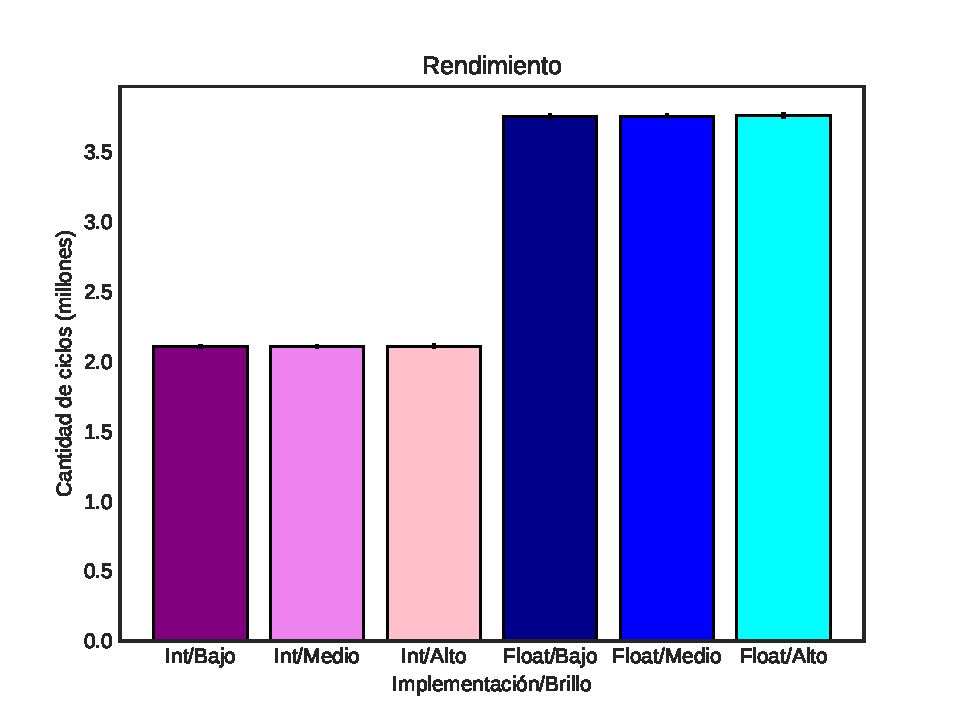
\includegraphics[scale=0.66]{img/IntvsFloat.pdf}
		\caption{Gráfico de barras de comparación de rendimiento.}		
\end{figure}
\justify
No se observan diferencias significativas en el rendimiento de una misma implementación en los diferentes casos, pero sí se puede notar un aumento del rendimiento de la implementación en enteros respecto a la de floats. 

\subsection{Experimento 2}
\justify
En el siguiente gráfico se resumen los resultados de la comparación por rendimiento entre las dos implementaciones de \textit{<<Reforzar Brillo>>}.

\begin{figure}[h]
	\centering
	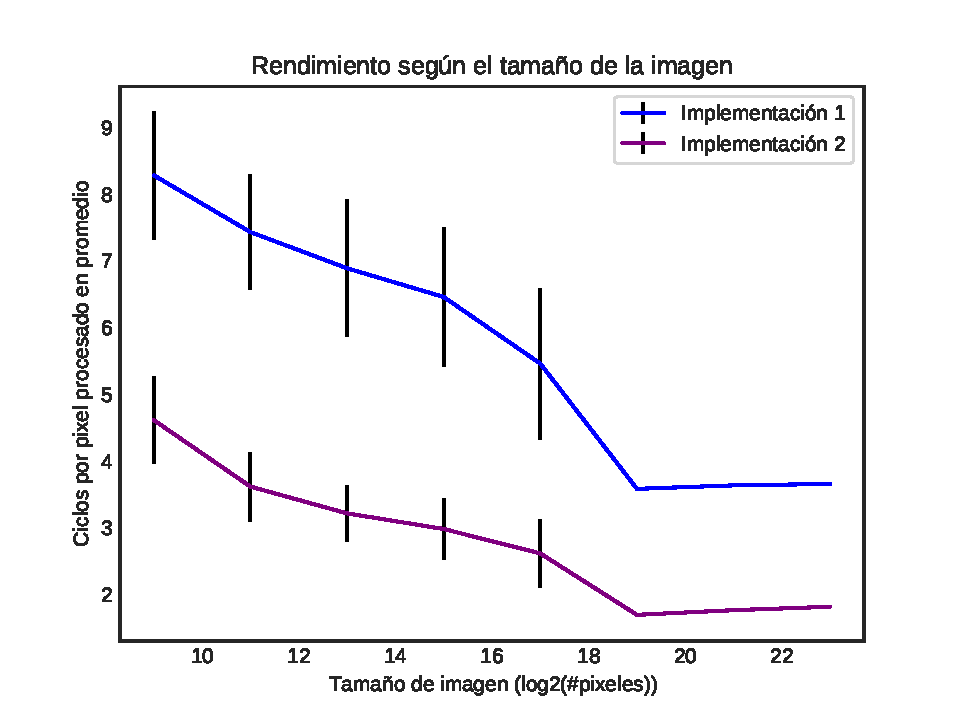
\includegraphics[scale=0.55]{img/ReforzarBrillo2vs4.pdf}
	\caption{Comparación de rendimiento en función del tamaño de la imagen.}
\end{figure}	
\justify
En ambos casos se observa la gráfica de una curva decreciente que se estanca a partir del tamaño 1024x512, similar a lo observado en resultados anteriores, aunque en este caso la curva es más empinada. Además, se puede notar una marcada diferencia entre el rendimiento de ambas implementaciones, siendo la segunda(cuatro píxeles procesados simultáneamente) la mejor y que la razón entre los tiempo de ejecución cuando los tamaños crecen tiende a 0.5. Por último, se puede observar nuevamente la extraña anomalía del desvío estándar que deja de tener valores significativos alrededor del tamaño mencionado anteriormente.

\section{Conclusión}
\justify
En primer lugar, a partir de los resultados del experimento \textit{<<Int vs Float para el filtro Imagen Fantasma>>}, se observa que las diferencias  entre operar con enteros y punto flotante residen principalmente en el rendimiento y en la precisión. Se puede concluir efectivamente que la pérdida de precisión no es significativa en ninguno de los dos casos y, en particular, la única implementación que pierde precisión es la de enteros. Esta pérdida es compensada con el hecho de que demora el 56\% de lo que demora la implementación con floats, reflejando una clara mejoría en el rendimiento. Esto coincide sastifactoriamente con la primera parte de nuestra hipótesis, la cual afirma que la implementación en enteros es mejor.
\justify
Por otro lado, la comparación para distintos tipos de brillo demuestra resultados coincidentes con la segunda parte de nuestra hipótesis que afirma que las imágenes con brillo medio son las que más precisión pierden, seguidas por las imágenes de brillo bajo. Y, en el caso de las imágenes con brillo alto, la pérdida de precisión es mucho menor debido a que las componentes se saturan con más facilidad. Además, podemos ver que estas comparaciones(rendimiento y precisión) son independientes, ya que en el gráfico de la Figura 18 no se observan diferencias entre el tiempo de ejecución variando el brillo de las imágenes. No obstante, podemos relacionarlas para concluir que la pérdida de precisión no es significativa en comparación con el rendimiento, en especial para los casos donde deban procesarse imágenes con brillo alto (pierde poca precisión por píxel) o bajo (la precisión que se pierde por componente es de a lo sumo una unidad), no así para las imágenes con brillo medio. 
\justify
En segundo lugar, los resultados del experimento \textit{<<Rendimiento en función de la cantidad de accesos a memoria y píxeles procesados para el filtro Reforzar Brillo>>} también son coincidentes con nuestra hipótesis. Como se observa en el gráfico de la Figura 19, la implementación que realiza menos accesos a memoria y procesa más píxeles en simultáneo (implementación 2), tiene un mejor rendimiento, es decir, es la más eficiente. Podemos afirmar que cuando el tamaño de la imagen supera la barrera de los $2^{19}$ píxeles, al no poseer un desvío estándar significativo en las muestras, la efectividad de la segunda implementación es el doble que el de la primera, confirmando nuestra hipótesis. 
\justify
En términos más generales, obtuvimos resultados contundentes que nos permitieron corroborar la efectividad de nuestras implementaciones en ASM con respecto a las implementaciones en C, por el uso de las instrucciones \textbf{SSE}, que nos permitieron procesar varios píxeles en simultáneo, llegando a poder demorar 2 ciclos por píxel, lo cuál se puede deber en gran parte a un procesador superescalar. Además, en los experimentos donde comparamos diferentes implementaciones en ASM, pudimos observar también una clara mejoría de rendimiento con tan solo buscar distintas instrucciones, o hacer un uso más eficiente de los registros \textit{xmm} (para el caso del experimento 2) que nos permitió levantar y procesar más píxeles en simultáneo, siempre manteniendo la idea original. 
\justify
Durante el transcurso del desarrollo de este informe se nos ocurrieron posibles lineas de investigación futuras con el fin de comprender mejor varios sucesos que nos ocurrieron durante las experimentaciones que nuestros resultados no llegaron a cubrirlos. Estos son:
\begin{itemize}
	\item  Investigar sobre las distintias optimizaciones de C para poder comprender en que casos se produce una mejoría del tiempo de ejecución, ya que a partir de nuestros resultados sólo se pudo observar una marcada diferencia entre O0 y las demás, pero no entre las últimas tres optimizaciones entre sí.
	\item Modificar las implementaciones hechas sobre ASM, con el fin de evitar la mayor cantidad de \textit{pipelines stalls} y así poder mejorar el tiempo de ejecución.
	\item Entender por qué ocurre la anomalía de los desvíos estándar cuando el tamaño de la imagen supera el número de $2^{19}$ píxeles.  
\end{itemize}  
\section{Anexo}
\subsection{Tablas de comparación C vs ASM}
\begin{table}[h!]
	\begin{center}
		\begin{tabular}{| l | c | c |}
			\hline
			Tamaño de Imagen & Media & Desviación estándar \\ \hline
			32x16	 & 5.921630859 &	0.9715292088 \\
			64x32	 & 4.927368164 & 0.7069422744 \\
			128x64	 & 4.348800659 & 0.6896616729 \\
			256x128	 & 4.068491364	& 0.5772964263 \\
			512x256	 & 3.29431057	& 0.6743555065 \\
			1024x512 & 2.219003534	& 0.0137942527 \\
			2048x1024 &	2.387156904	& 0.01624362425 \\ \hline
		\end{tabular}
		\caption{Tabla de media y desvío estándar de la implementación en ASM del filtro Imagen Fantasma}
	\end{center}
\end{table}

\begin{table}[h!]
	\begin{center}
		\begin{tabular}{| l | c | c |}
			\hline
			Tamaño de Imagen & Media & Desviación estándar \\ \hline
			32x16	& 81.47636719	& 11.09416675 \\
			64x32	& 81.37869873	& 9.728125887 \\
			128x64	& 72.43599243	& 11.04824393 \\
			256x128	& 62.6981987	& 9.284730169 \\
			512x256	& 45.280196	& 9.93687337 \\
			1024x512 & 29.50892844	& 0.1147064117 \\
			2048x1024 & 28.35182894	& 0.1511577683 \\ \hline
		\end{tabular}
		\caption{Tabla de media y desvío estándar de la implementación en C-O3 del filtro Imagen Fantasma}
	\end{center}
\end{table}

\begin{table}[h!]
	\begin{center}
		\begin{tabular}{| l | c | c |}
			\hline
			Tamaño de Imagen & Media & Desviación estándar \\ \hline
			32x16	& 97.62231445	& 12.06571904 \\
			64x32	& 98.07945557	& 13.35950448 \\ 
			128x64	& 98.60905151	& 13.54354344 \\
			256x128	& 90.24432907	& 13.34403614 \\
			512x256	& 67.98446102	& 12.88308288 \\
			1024x512 & 41.91469574	& 0.1226711478 \\
			2048x1024 &41.15305513	& 0.2141665253 \\ \hline
		\end{tabular}
		\caption{Tabla de media y desvío estándar de la implementación en C-O3 del filtro Color Bordes}
	\end{center}
\end{table}


\begin{table}[h!]
	\begin{center}
		\begin{tabular}{| l | c | c |}
			\hline
			Tamaño de Imagen & Media & Desviación estándar \\ \hline
			32x16	& 8.650195313	& 0.9721211703 \\
			64x32	& 7.945532227	& 0.9825540828 \\
			128x64	& 7.540411377	& 1.194941323 \\
			256x128	& 7.572285461	& 1.093124848 \\
			512x256	& 6.16046505	& 1.328212482 \\
			1024x512 & 4.223790836	& 0.01833876837 \\
			2048x1024 &4.322357082	& 0.02027162607 \\ \hline
		\end{tabular}
		\caption{Tabla de media y desvío estándar de la implementación en ASM del filtro Color Bordes}
	\end{center}
\end{table}
\newpage
\begin{table}[h!]
	\begin{center}
		\begin{tabular}{| l | c | c |}
			\hline
			Tamaño de Imagen & Media & Desviación estándar \\ \hline
			32x16	& 34.81259766	& 3.888256511 \\
			64x32	& 34.58880615	& 4.757211972 \\
			128x64	& 33.37852478	& 4.559472662 \\
			256x128	& 28.26952515	& 4.424189227 \\
			512x256	& 20.09854145	& 4.382768938 \\
			1024x512 & 12.57793593	& 0.1222174024 \\
			2048x1024 & 11.82362655	& 0.132867672 \\ \hline 
		\end{tabular}
		\caption{Tabla de media y desvío estándar de la implementación en C-O3 del filtro Reforzar Brillo}
	\end{center}
\end{table}

\begin{table}[h!]
	\begin{center}
		\begin{tabular}{| l | c | c |}
			\hline
			Tamaño de Imagen & Media & Desviación estándar \\ \hline
			32x16	& 4.544384766	& 0.6066059132 \\
			64x32	& 3.597692871	 & 0.5132170263 \\
			128x64	& 3.249700928	& 0.4674604985 \\
			256x128	& 3.023780823	& 0.4825971645 \\
			512x256	& 2.525241852	& 0.5421874291 \\
			1024x512 & 1.69808507	& 0.008867189432\\ 
			2048x1024 & 1.778618181	& 0.007530822535 \\ \hline
		\end{tabular}
		\caption{Tabla de media y desvío estándar de la implementación en ASM del filtro Reforzar Brillo}
	\end{center}
\end{table}

\subsection{Tablas experimento 1}

\begin{table}[h!]
	\begin{center}
		\begin{tabular}{| l | c | c |}
			\hline
			Brillo de Imagen & Media & Desviación estándar \\ \hline
			Brillo Bajo	& 2107123.425	& 15524.49565 \\
			Brillo Medio &	2103910.425	& 14988.86603 \\
			Brillo Alto	& 2107895.625	& 15552.71122 \\ \hline
		\end{tabular}
		\caption{Tabla de media y desvío estándar de la implementación en Imagen Fantasma con enteros}
	\end{center}
\end{table}

\begin{table}[h!]
	\begin{center}
		\begin{tabular}{| l | c | c |}
			\hline
			Brillo de Imagen & Media & Desviación estándar \\ \hline
			Brillo  Bajo	& 3750866.1	& 20012.27356 \\
			Brillo Medio	& 3752772.975	& 19529.32267 \\
			Brillo Alto	& 3754959.525 &	21985.43382 \\ \hline
		\end{tabular}
		\caption{Tabla de media y desvío estándar de la implementación en Imagen Fantasma con floats}
	\end{center}
\end{table}

\newpage
\subsection{Tablas experimento 2}

\begin{table}[h!]
	\begin{center}
		\begin{tabular}{| l | c | c |}
			\hline
			Tamaño de Imagen & Media & Desviación estándar \\ \hline
			32x16	& 4.614257813	& 0.6489414646 \\
			64x32	& 3.618786621	& 0.5184705916 \\
			128x64	& 3.2181427	& 0.422223637 \\
			256x128	& 2.984065247	& 0.4543680938 \\
			512x256	& 2.617810249	& 0.5154508241 \\
			1024x512	& 1.698392344	& 0.01136544077 \\
			2048x1024	& 1.768280625	& 0.007083708599 \\
			4096x2048	& 1.819600832	& 0.00623151489\\ \hline
		\end{tabular}
		\caption{Tabla de media y desvío estándar de la implementación de Reforzar Brillo con 4 píxeles}
	\end{center}
\end{table}

\begin{table}[h!]
	\begin{center}
		\begin{tabular}{| l | c | c |}
			\hline
			Tamaño de Imagen & Media & Desviación estándar \\ \hline
			32x16	& 8.280615234	& 0.9547151406 \\
			64x32	& 7.430712891	& 0.8593684381 \\
			128x64	& 6.888757324	& 1.028142185 \\
			256x128	& 6.459040833	& 1.041688197 \\
			512x256	& 5.460948372	& 1.132243435 \\
			1024x512	& 3.585107946	& 0.01980786682 \\
			2048x1024	& 3.63749181	& 0.01056004466 \\
			4096x2048	& 3.658681422	& 0.01361814104 \\ \hline
		\end{tabular}
		\caption{Tabla de media y desvío estándar de la implementación de Reforzar Brillo con 2 píxeles}
	\end{center}
\end{table}

%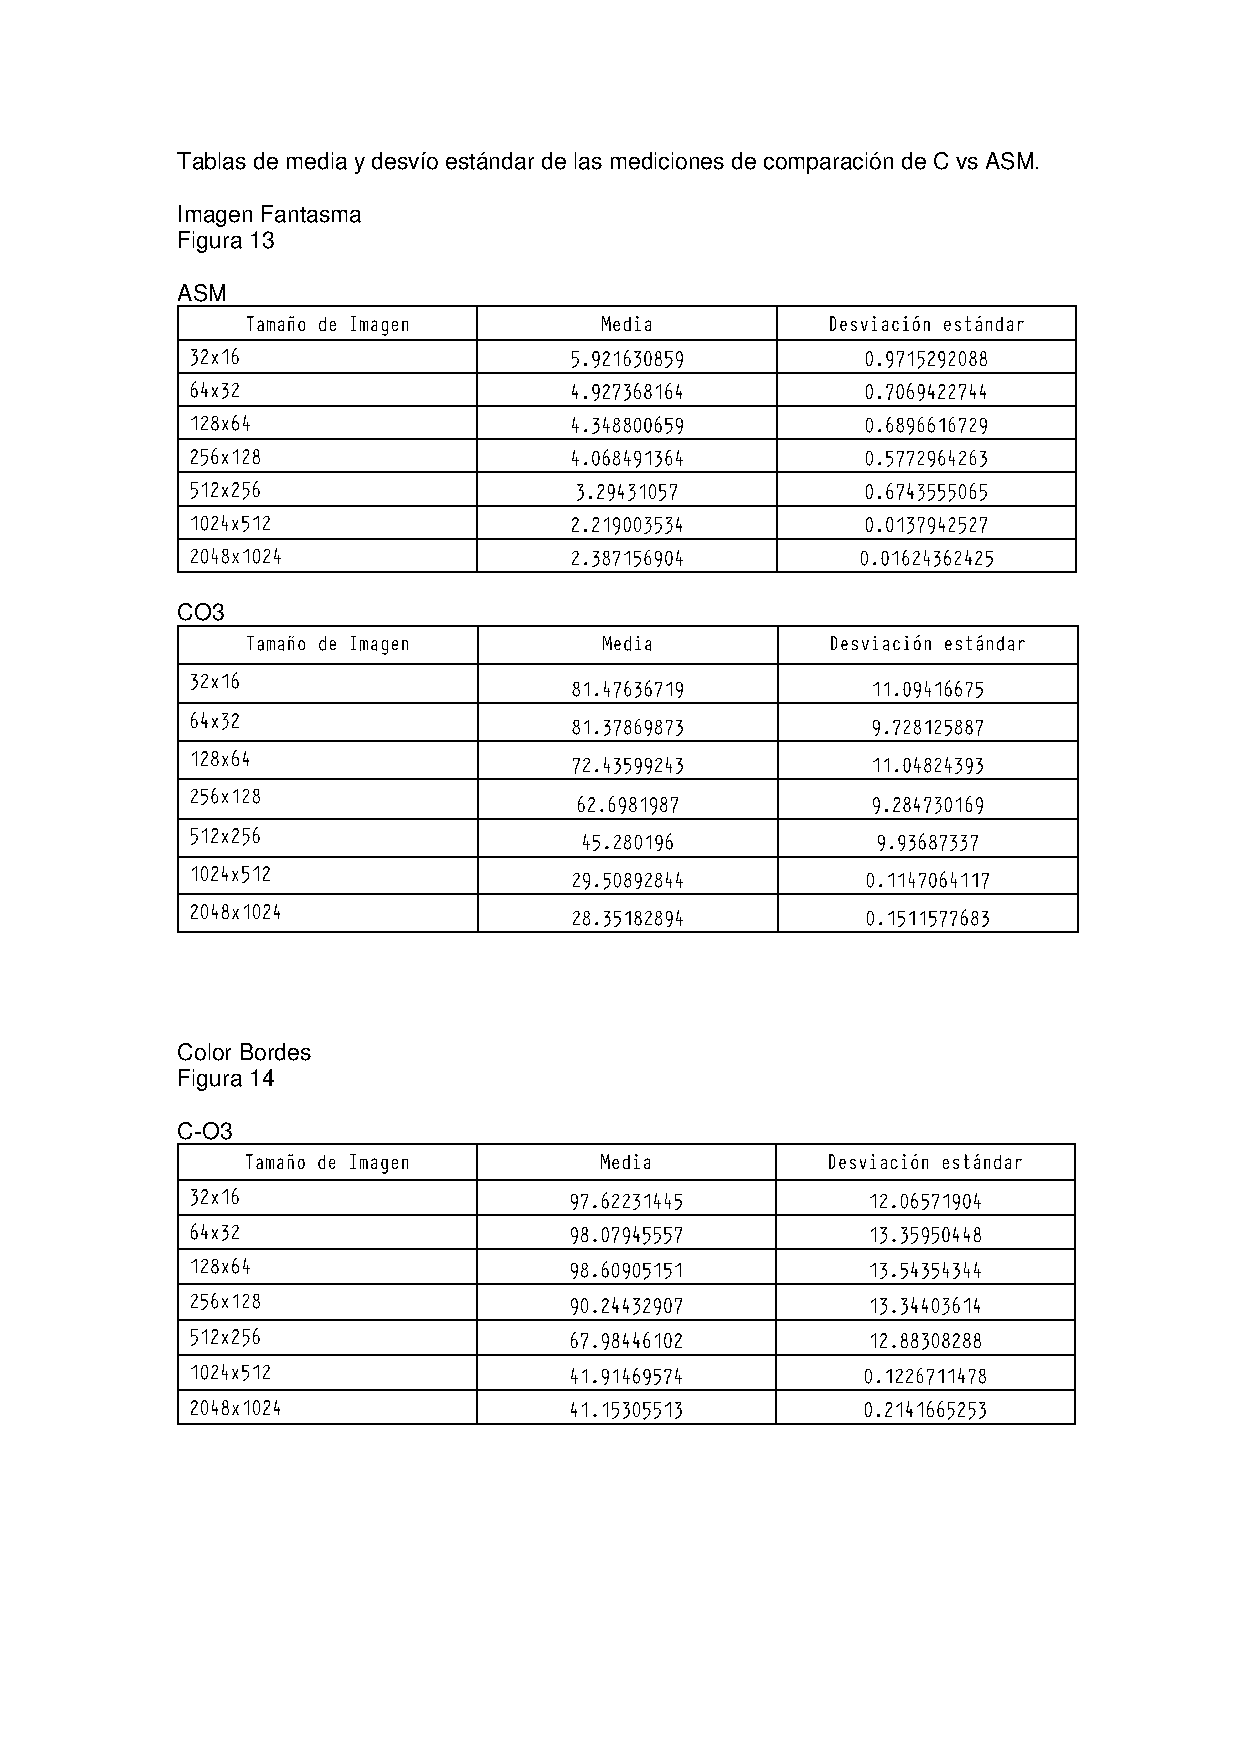
\includepdf[pages=-]{img/Tablas.pdf}
\end{document}

